\documentclass{llncs}

\usepackage{amsmath,amssymb,amsfonts}
\usepackage{graphicx}
\usepackage{xcolor, colortbl}
\usepackage{stmaryrd}
\usepackage{subcaption}
\usepackage{hyperref}
\usepackage[capitalize]{cleveref}
\usepackage{tikz}

\usetikzlibrary{automata,positioning,shapes.multipart,arrows.meta}

\title{Flexible Runtime Security Enforcement with Tagged C}
\author{Sean Anderson \and Allison Naaktgeboren \and Andrew Tolmach}
\institute{Portland State University}

\begin{document}

\newcommand{\tagcolor}{C}

\newcommand{\vt}{\mathit{vt}}
\newcommand{\pt}{\mathit{pt}}
\newcommand{\lt}{\mathit{lt}}
\newcommand{\lts}{\overline{\lt}}
\newcommand{\nt}{\mathit{nt}}
\newcommand{\PCT}{\mathcal{P}}

\newcommand{\trule}[2]{#1 \leftarrow #2}

\newcommand{\truledef}[1]{
  & \multispan{3} \(#1\) \\}

\newcommand{\assert}[1]{& & & \multispan{2} \(\mathbf{assert} ~ #1\) \hfill \\}
\newcommand{\letin}[1]{& & & \multispan{2} \(\mathit{let} ~ #1 ~ \mathit{in}\) \\}

\newcommand{\caseof}[1]{\textnormal{case } #1 \textnormal{ of}}
\newcommand{\caseentry}[2]{& & & #1 \Rightarrow #2}

\newcommand{\optional}[1]{\fcolorbox{black}{gray!20}{#1}}
\newcommand{\settag}[2]{\boldsymbol{#1} & \longleftarrow & & \mathit{#2}\\}
\newcommand{\settagopt}[2]{\optional{\(\boldsymbol{#1}\)} & \longleftarrow & & \mathit{#2}\\}

%%% Tag Rules %%%
\newcommand{\loadtname}{\mathbf{LoadT}}
\newcommand{\loadtargs}{\PCT, \pt, \vt, \overline{\lt}}
\newcommand{\loadtres}{\vt'}
\newcommand{\loadt}{\loadtname(\loadtargs)}

\newcommand{\storetname}{\mathbf{StoreT}}
\newcommand{\storetargs}{\PCT, \pt, \vt_1, \vt_2, \overline{\lt}}
\newcommand{\storetres}{\PCT',\vt',\overline{\lt}'}
\newcommand{\storet}{\storetname(\storetargs)}

\newcommand{\consttname}{\mathbf{ConstT}}
\newcommand{\consttres}{\vt}
\newcommand{\constt}{\consttname}

\newcommand{\unoptname}{\mathbf{UnopT}}
\newcommand{\unoptargs}{\PCT, \vt}
\newcommand{\unoptres}{\vt}
\newcommand{\unopt}{\unoptname(\unoptargs)}

\newcommand{\binoptname}{\mathbf{BinopT}}
\newcommand{\binoptargs}{\PCT, \vt_1, \vt_2}
\newcommand{\binoptres}{\vt'}
\newcommand{\binopt}{\binoptname(\binoptargs)}

\newcommand{\globaltname}{\mathbf{GlobalT}}
\newcommand{\globaltargs}{id, s}
\newcommand{\globaltargstyped}{id \in ident, s \in \mathbb{N}}
\newcommand{\globaltres}{\pt,\vt,\overline{\lt}}
\newcommand{\globalt}{\globaltname(\globaltargs)}

\newcommand{\localtname}{\mathbf{LocalT}}
\newcommand{\localtargs}{\PCT, id, s}
\newcommand{\localtargstyped}{\PCT, id \in ident, s \in \mathbb{N}}
\newcommand{\localtres}{\pt,\vt,\overline{\lt}}
\newcommand{\localt}{\localtname(\localtargs)}

\newcommand{\vartname}{\mathbf{VarT}}
\newcommand{\vartargs}{\PCT, \vt}
\newcommand{\vartres}{\pt}
\newcommand{\vart}{\vartname(\vartargs)}

\newcommand{\malloctname}{\mathbf{MallocT}}
\newcommand{\malloctargs}{\PCT, \vt}
\newcommand{\malloctres}{\PCT',\pt,\optional{\(\vt,\overline{\lt}\)}}
\newcommand{\malloct}{\malloctname(\malloctargs)}

\newcommand{\freetname}{\mathbf{FreeT}}
\newcommand{\freetargs}{\PCT, \vt}
\newcommand{\freetres}{\PCT',\pt,\optional{\(\vt,\overline{\lt}\)}}
\newcommand{\freet}{\freetname(\freetargs)}

\newcommand{\picasttname}{\mathbf{PICastT}}
\newcommand{\picasttargs}{\PCT, \pt, \optional{\(\vt, \overline{\lt}\)}}
\newcommand{\picasttres}{\PCT',\vt}
\newcommand{\picastt}{\picasttname(\picasttargs)}

\newcommand{\ipcasttname}{\mathbf{IPCastT}}
\newcommand{\ipcasttargs}{\PCT, \vt_1, \optional{\(\vt_2, \overline{\lt}\)}}
\newcommand{\ipcasttres}{\PCT',\pt}
\newcommand{\ipcastt}{\ipcasttname(\ipcasttargs)}

\newcommand{\ppcasttname}{\mathbf{PPCastT}}
\newcommand{\ppcasttargs}{\PCT, \pt, \optional{\(\vt, \overline{\lt}\)}}
\newcommand{\ppcasttres}{\PCT',\pt'}
\newcommand{\ppcastt}{\picasttname(\picasttargs)}

\newcommand{\iicasttname}{\mathbf{IICastT}}
\newcommand{\iicasttargs}{\PCT, \vt_1}
\newcommand{\iicasttres}{\PCT',\pt}
\newcommand{\iicastt}{\ipcasttname(\ipcasttargs)}

\newcommand{\splittname}{\mathbf{SplitT}}
\newcommand{\splittargs}{\PCT, \vt, \optional{\(L\)}}
\newcommand{\splittres}{\PCT'}
\newcommand{\splitt}{\splittname(\splittargs)}
           
\newcommand{\jointname}{\mathbf{JointT}}
\newcommand{\jointargs}{\PCT, \optional{\(L\)}}
\newcommand{\jointres}{\PCT'}
\newcommand{\joint}{\jointname(\jointargs)}

\newcommand{\argtname}{\mathbf{ArgT}}
\newcommand{\argtargs}{\PCT, \vt, f, x}
\newcommand{\argtargstyped}{\PCT, \vt, f, x \in ident}
\newcommand{\argtres}{\vt'}
\newcommand{\argt}{\argtname(\argtargs)}

\newcommand{\callerrettname}{\mathbf{CallerRetT}}
\newcommand{\callerrettargs}{\PCT, \PCT', \vt}
\newcommand{\callerrettres}{\vt'}
\newcommand{\callerrett}{\callerrettname(\callerrettargs)}

\newcommand{\calleerettname}{\mathbf{CalleeRetT}}
\newcommand{\calleerettargs}{\PCT, \PCT', \vt}
\newcommand{\calleerettres}{\vt'}
\newcommand{\calleerett}{\calleerettname(\calleerettargs)}

%%%%%%%%%%%%%%%%%

%%% Continuations, States, Values %%%

\newcommand{\kemp}{\mathit{Kemp}}
\newcommand{\kdo}[1]{\mathit{Kdo};~ #1}
\newcommand{\kseq}[2]{\mathit{Kseq} ~ #1; ~ #2}
\newcommand{\kif}[4]{\mathit{Kif}[#1 \mid #2] ~ \mathit{join} ~ #3; ~ #4}
\newcommand{\kwhiletest}[4]{\mathit{KwhileTest}(#1) ~ \{ ~ #2 ~ \} ~ \mathit{join} ~ #3; ~ #4}
\newcommand{\kwhileloop}[4]{\mathit{KwhileLoop}(#1) ~ \{ ~ #2 ~ \} ~ \mathit{join} ~ #3; ~ #4}
\newcommand{\kdowhiletest}[4]{\mathit{KdoWhileTest}(#1) ~ \{ ~ #2 ~ \} ~ \mathit{join} ~ #3; ~ #4}
\newcommand{\kdowhileloop}[4]{\mathit{KdoWhileLoop}(#1) ~ \{ ~ #2 ~ \} ~ \mathit{join} ~ #3; ~ #4}
\newcommand{\kfor}[2]{\mathit{Kfor} ~ #1; ~ #2}
\newcommand{\kforpost}[2]{\mathit{KforPost} ~ #1; ~ #2}
\newcommand{\kcall}[3]{\mathit{Kcall} ~ #1 ~ #2 ~ #3}

\newcommand{\ctx}[1]{ctx \left[#1\right]}

\newcommand{\sstate}[6]{\mathcal{S}\left(f,#2,#3,#4 \mid #5 \gg #6 @ #1\right)}
\newcommand{\estate}[6]{\mathcal{E}\left(f,#2,#3,#4 \mid #5; \gg #6 @ #1\right)}
\newcommand{\cstate}[7]{\mathcal{C}\left(#1,#3,#4 \mid #5(#6) \gg #7 @ #2\right)}
\newcommand{\rstate}[6]{\mathcal{R}\left(#1,#3,#4 \mid #5 \gg #6 @ #2\right)}
\newcommand{\fstate}[1]{\mathcal{F}\left(#1\right)}

\newcommand{\mem}{m}
\newcommand{\genv}{\mathit{ge}}
\newcommand{\lenv}{\mathit{le}}
\newcommand{\cont}{k}
\newcommand{\stmt}{s}
\newcommand{\expr}{e}
\newcommand{\type}{ty}
\newcommand{\defestate}[1]
           {\estate{\PCT}{\mem}{\genv}{\lenv}{#1}{\cont}}
\newcommand{\defsstate}[1]
           {\sstate{\PCT}{\mem}{\genv}{\lenv}{#1}{\cont}}

\newcommand{\valof}[1]{|#1|}
\newcommand{\deref}[1]{* #1}
\newcommand{\addrof}[1]{\& #1}
\newcommand{\assignop}[3]{#2 ~~ [#1]\!\!= #3}
\newcommand{\postinc}[2]{#2 #1\!\!#1}
\newcommand{\assign}[2]{#1 := #2}
\newcommand{\loc}[2]{\underline{#1}@#2}
\newcommand{\val}[2]{\mathit{#1} @ #2}
\newcommand{\binop}[3]{#2 #1 #3}
\newcommand{\unop}[2]{#1 #2}
\newcommand{\comma}[2]{#1, #2}
\newcommand{\paren}[2]{(#2) (#1)}
\newcommand{\builtin}[2]{\mathit{builtin} ~ #1(#2)}
\newcommand{\var}[1]{#1}
\newcommand{\cast}[2]{(#2) #1}
\newcommand{\call}[2]{#1(#2)}
\newcommand{\condition}[3]{#1 ~ ? ~ #2 ~ : ~ #3}
\newcommand{\sizeof}[1]{\mathtt{size}(#1)}
\newcommand{\alignof}[1]{\mathtt{align}(#1)}

\newcommand{\sskip}{\mathtt{skip}}
\newcommand{\sdo}[1]{#1;}
\newcommand{\sseq}[2]{#1 ~ #2}
\newcommand{\scontinue}{\mathtt{continue}}
\newcommand{\sbreak}{\mathtt{break}}
\newcommand{\sreturn}{\mathtt{return}}
\newcommand{\sifthenelse}[4]{\mathtt{if}(#1) ~ \mathtt{then} ~ #2 ~ \mathtt{else} ~ #3 ~ \mathtt{join} ~ #4}
\newcommand{\swhile}[3]{\mathtt{while}(#1) ~ \mathtt{do} ~ #2 ~ \mathtt{join} ~ #3}
\newcommand{\sdowhile}[3]{\mathtt{do} ~ #2 ~ \mathtt{while} ~ (#1) ~ \mathtt{join} ~ #3}
\newcommand{\sfor}[5]{\mathtt{for}(#1; #2; #3) ~ \mathtt{do} ~ #4 ~ \mathtt{join} ~ #5}
\newcommand{\sswitch}[2]{\mathtt{switch} ~ #1 ~ \{ ~ #2 ~ \}}
\newcommand{\slabel}[2]{#1: ~ #2}
\newcommand{\sgoto}[1]{\mathtt{goto} ~ #1}

\newcommand{\vundef}{\mathbf{undef}}

\newcommand{\tptr}[1]{\mathit{ptr(#1)}}

\newcommand{\judgment}[3][]{
  {\centering
  \smallskip
  \begin{tabular}{c}
    #2 \\
    \hline
    #3
  \end{tabular}{\sc #1}
  \smallskip\par}}

\newcommand{\judgmentbr}[4][]{
  {\centering
  \smallskip
  \begin{tabular}{c}
    #2 \\
    #3 \\
    \hline
    #4
  \end{tabular}{\sc #1}
   \smallskip\par}}

\newcommand{\judgmentbrbr}[5][]{
  {\centering
  \smallskip
  \begin{tabular}{c}
    #2 \\
    #3 \\
    #4 \\
    \hline
    #5
  \end{tabular}{\sc #1}
   \smallskip\par}}

\newcommand{\judgmentbrbrbr}[6][]{
  {\centering
  \smallskip
  \begin{tabular}{c}
    #2 \\
    #3 \\
    #4 \\
    #5 \\
    \hline
    #6
  \end{tabular}{\sc #1}
   \smallskip\par}}

\newcommand{\judgmenttwobr}[6][]{
  {
    \centering
    \smallskip
    \begin{tabular}{c c}
       #2 & #3 \\
       #4 & #5 \\
       \hline
       \multicolumn{2}{c}{#6}
    \end{tabular}{\sc #1}
    \vspace{\belowdisplayskip}\par
  }}

\newcommand{\judgmenttwobrlong}[5][]{
  {
    \centering
    \smallskip
    \begin{tabular}{c c}
       #2 & #3 \\
       \multicolumn{2}{c}{#4} \\
       \hline
       \multicolumn{2}{c}{#5}
    \end{tabular}{\sc #1}
    \vspace{\belowdisplayskip}\par
  }}

\newcommand{\judgmentthreebrlong}[6][]{
  {
    \centering
    \smallskip
    \begin{tabular}{c c c}
       #2 & #3 & #4 \\
       \multicolumn{3}{c}{#5} \\
       \hline
       \multicolumn{3}{c}{#6}
    \end{tabular}{\sc #1}
    \vspace{\belowdisplayskip}\par
  }}

\newcommand{\judgmentthreebrtwo}[7][]{
  {
    \centering
    \smallskip
    \begin{tabular}{c c c}
       #2 & #3 & #4 \\
       \multicolumn{3}{c}{#5 \hfill #6} \\
       \hline
       \multicolumn{3}{c}{#7}
    \end{tabular}{\sc #1}
    \vspace{\belowdisplayskip}\par
  }}

\newcommand{\judgmenttwobrlongbrlong}[6][]{
  {
    \centering
    \smallskip
    \begin{tabular}{c c}
       #2 & #3 \\
       \multicolumn{2}{c}{#4} \\
       \multicolumn{2}{c}{#5} \\
       \hline
       \multicolumn{2}{c}{#6} \\
    \end{tabular}{\sc #1}
    \vspace{\belowdisplayskip}\par
  }}


\newcommand{\judgmentthreebr}[8][]{
  {
    \centering
    \smallskip
    \begin{tabular}{c c c}
       #2 & #3 & #4 \\
       #5 & #6 & #7 \\
       \hline
       \multicolumn{3}{c}{#8}
    \end{tabular}{\sc #1}
    \vspace{\belowdisplayskip}\par
  }}


\newcommand{\judgmenttwo}[4][]{
  {\centering
  \smallskip
  \begin{tabular}{c c}
    #2 & #3 \\
    \hline
    \multicolumn{2}{c}{#4}
  \end{tabular}{\sc #1}
  \smallskip\par}}

\newcommand{\judgmentthree}[5][]{
  {\centering
  \smallskip
  \begin{tabular}{c c c}
    #2 & #3 & #4 \\
    \hline
    \multicolumn{3}{c}{#5}
  \end{tabular}{\sc #1}
  \smallskip\par}}

\newcommand{\judgmentfour}[6][]{
  {\centering
  \smallskip
  \begin{tabular}{c c c c}
    #2 & #3 & #4 & #5 \\
    \hline
    \multicolumn{4}{c}{#6}
  \end{tabular}{\sc #1}
  \smallskip\par}}

\newcommand{\truleblock}[2]
           {
             \tcbox{
             \begin{tabular}{l}
               #1 \\
               #2 \\
             \end{tabular}}
           }

\newcommand{\malloctname}{\color{blue} \mathbf{MallocT}}
\newcommand{\malloctargs}{\PCT, \pt, \vt}
\newcommand{\malloctres}{\PCT['],\pt['],\vt['],\lt[']}
\newcommand{\malloct}{\malloctname(\malloctargs)}

\newcommand{\malloctruleblock}[1]
           {
             \truleblock{\(\malloct\)}{#1}
           }

\newcommand{\localtname}{\color{blue} \mathbf{LocalT}}
\newcommand{\localtargs}{\PCT, \TN}
\newcommand{\localtres}{\PCT['], \pt['], \lt[']}
\newcommand{\localt}{\localtname(\localtargs)}

\newcommand{\localtruleblock}[1]
           {
             \truleblock{\(\localt\)}{#1}
           }

\newcommand{\accesstname}{\color{blue} \mathbf{AccessT}}
\newcommand{\accesstargs}{\PCT,\vt}
\newcommand{\accesstres}{\vt[']}
\newcommand{\accesst}{\accesstname(\accesstargs)}

\newcommand{\accesstruleblock}[1]
           {
             \truleblock{\(\accesst\)}{#1}
           }

\newcommand{\loadtname}{\color{blue} \mathbf{LoadT}}
\newcommand{\loadtargs}{\PCT, \pt, \vt, \lt}
\newcommand{\loadtres}{\vt[']}
\newcommand{\loadt}{\loadtname(\loadtargs)}

\newcommand{\loadtruleblock}[1]
           {
             \truleblock{\(\loadt\)}{#1}
           }

\newcommand{\assigntname}{\color{blue} \mathbf{AssignT}}
\newcommand{\assigntargs}{\PCT,\vt[_1],\vt[_2]}
\newcommand{\assigntres}{\PCT['],\vt[']}
\newcommand{\assignt}{\assigntname(\assigntargs)}

\newcommand{\assigntruleblock}[1]
           {
             \truleblock{\(\assignt\)}{#1}
           }
           
\newcommand{\storetname}{\color{blue} \mathbf{StoreT}}
\newcommand{\storetargs}{\PCT, \pt, \vt, \lt}
\newcommand{\storetres}{\PCT['],\vt['],\lt[']}
\newcommand{\storet}{\storetname(\storetargs)}

\newcommand{\storetruleblock}[1]
           {
             \truleblock{\(\storet\)}{#1}
           }

\newcommand{\unoptname}{\color{blue} \mathbf{UnopT}}
\newcommand{\unoptargs}{\odot, \PCT, \vt}
\newcommand{\unoptres}{\vt[']}
\newcommand{\unopt}{\unoptname(\unoptargs)}
           
\newcommand{\unoptruleblock}[2]
           {
             \colorbox{blue!10}{
               \begin{tabular}{l}
                 \(\unopt\) \\
                 % body
                 #1 \\
                 % outputs
                 \{ \(\unoptres\) \} \\
               \end{tabular}
             }
           }
           
\newcommand{\binoptname}{\color{blue} \mathbf{BinopT}}
\newcommand{\binoptargs}{\oplus, \PCT, \vt[_1], \vt[_2]}
\newcommand{\binoptexargs}{\oplus,\vt[_1],\vt[_2]}
\newcommand{\binoptres}{\vt[']}
\newcommand{\binopt}{\binoptname(\binoptargs)}
\newcommand{\binoptex}{\binoptname(\binoptexargs)}

\newcommand{\binoptruleblock}[1]
           {
             \truleblock{\(\binopt\)}{#1}
           }

\newcommand{\binoptexruleblock}[1]
           {
             \truleblock{\(\binoptex\)}{#1}
           }

           
\newcommand{\calltname}{\color{blue} \mathbf{CallT}}
\newcommand{\calltargs}{\PCT, \pt}
\newcommand{\calltres}{\PCT[']}
\newcommand{\callt}{\calltname(\calltargs)}
           
\newcommand{\calltruleblock}[1]
           {
             \truleblock{\(\callt\)}{#1}
           }

\newcommand{\argtname}{\color{blue} \mathbf{ArgT}}
\newcommand{\argtargs}{\PCT, \vt, \FN, \AN}
\newcommand{\argtexargs}{\vt,\FN,\AN}
\newcommand{\argtres}{\PCT['], \vt[']}
\newcommand{\argt}{\argtname(\argtargs)}
\newcommand{\argtex}{\argtname(\argtexargs)}

\newcommand{\argtruleblock}[1]
           {
             \truleblock{\(\argt\)}{#1}
           }

\newcommand{\argtexruleblock}[1]
           {
             \truleblock{\(\argtex\)}{#1}
           }
           
\newcommand{\rettname}{\color{blue} \mathbf{RetT}}
\newcommand{\rettargs}{\PCT[_{\color{blue} CLE}], \PCT[_{\color{blue} CLR}], \vt}
\newcommand{\rettres}{\PCT['],\vt[']}
\newcommand{\rett}{\rettname(\rettargs)}

\newcommand{\rettruleblock}[1]
           {
             \truleblock{\(\rett\)}{#1}
           }

\newcommand{\consttname}{\color{blue} \mathbf{ConstT}}
\newcommand{\consttargs}{\PCT}
\newcommand{\consttres}{\vt[']}
\newcommand{\constt}{\consttname(\consttargs)}

\newcommand{\consttruleblock}[1]
           {
             \truleblock{\(\constt\)}{#1}
           }

\newcommand{\inittname}{{\color{blue} \mathbf{InitT}}}
\newcommand{\inittargs}{\PCT}
\newcommand{\inittres}{\vt[']}
\newcommand{\initt}{\inittname(\inittargs)}

\newcommand{\inittruleblock}[1]
           {
             \truleblock{\(\initt\)}{#1}
           }
           
\newcommand{\globaltname}{\color{blue} \mathbf{GlobalT}}
\newcommand{\globaltargs}{\GN, \TN}
\newcommand{\globaltres}{\pt['],\vt['],\lt[']}
\newcommand{\globalt}{\globaltname(\globaltargs)}

\newcommand{\globaltruleblock}[1]
           {
             \truleblock{\(\globalt\)}{#1}
           }

\newcommand{\dealloctname}{\color{blue} \mathbf{DeallocT}}
\newcommand{\dealloctargs}{\PCT, \TN}
\newcommand{\dealloctres}{\PCT['],\vt['],\lt[']}
\newcommand{\dealloct}{\dealloctname(\dealloctargs)}

\newcommand{\freetname}{\color{blue} \mathbf{FreeT}}
\newcommand{\freetargs}{\PCT,\pt,\vt}
\newcommand{\freetres}{\PCT['],\vt['],\lt[']}
\newcommand{\freet}{\freetname(\freetargs)}

\newcommand{\picasttname}{\color{blue} \mathbf{PICastT}}
\newcommand{\picasttargs}{\PCT, \pt, \lt, \TN}
\newcommand{\picasttres}{\vt[']}
\newcommand{\picastt}{\picasttname(\picasttargs)}

\newcommand{\picasttruleblock}[1]
           {
             \truleblock{\(\picastt\)}{#1}
           }

\newcommand{\ipcasttname}{\color{blue} \mathbf{IPCastT}}
\newcommand{\ipcasttargs}{\PCT, \vt, \lt, \TN}
\newcommand{\ipcasttres}{\pt[']}
\newcommand{\ipcastt}{\ipcasttname(\ipcasttargs)}

\newcommand{\ipcasttruleblock}[1]
           {
             \truleblock{\(\ipcastt\)}{#1}
           }

\newcommand{\ppcasttname}{\color{blue} \mathbf{PPCastT}}
\newcommand{\ppcasttargs}{\PCT, \pt[_1], \pt[_2], \lt[_1], \lt[_2], \TN}
\newcommand{\ppcasttres}{\pt[']}
\newcommand{\ppcastt}{\ppcasttname(\ppcasttargs)}

\newcommand{\iicasttname}{\color{blue} \mathbf{IICastT}}
\newcommand{\iicasttargs}{\PCT, \vt[_1], \TN}
\newcommand{\iicasttres}{\pt[']}
\newcommand{\iicastt}{\iicasttname(\iicasttargs)}

\newcommand{\splittname}{\color{blue} \mathbf{SplitT}}
\newcommand{\splittargs}{\PCT, \vt, \LN}
\newcommand{\splittres}{\PCT[']}
\newcommand{\splitt}{\splittname(\splittargs)}

\newcommand{\splittruleblock}[1]
           {
             \truleblock{\(\splitt\)}{#1}
           }

\newcommand{\exprsplittname}{\color{blue} \mathbf{ExprSplitT}}
\newcommand{\exprsplittargs}{\PCT, \vt}
\newcommand{\exprsplittres}{\PCT[']}
\newcommand{\exprsplitt}{\exprsplittname(\exprsplittargs)}

\newcommand{\exprsplittruleblock}[1]
           {
             \colorbox{blue!10}{
               \begin{tabular}{l}
                 \(\exprsplitt\) \\
                 #1 \\
               \end{tabular}
             }
           }


\newcommand{\exprjointname}{\color{blue} \mathbf{ExprJoinT}}
\newcommand{\exprjointargs}{\PCT, \vt}
\newcommand{\exprjointres}{\PCT['], \vt[']}
\newcommand{\exprjoint}{\exprjointname(\exprjointargs)}

\newcommand{\exprjointruleblock}[1]
           {
             \colorbox{blue!10}{
               \begin{tabular}{l}
                 \(\exprjoint\) \\
                 #1 \\
               \end{tabular}
             }
           }

\newcommand{\labeltname}{\color{blue} \mathbf{LabelT}}
\newcommand{\labeltargs}{\PCT, \LN}
\newcommand{\labeltres}{\PCT[']}
\newcommand{\labelt}{\labeltname(\labeltargs)}

\newcommand{\labeltruleblock}[1]
           {
             \truleblock{\(\labelt\)}{#1}
           }

\newcommand{\extcalltname}{\color{blue} \mathbf{ExtCallT}}
\newcommand{\extcalltargs}{\PCT, \pt, \overline{\vt}}
\newcommand{\extcalltres}{\PCT[']}
\newcommand{\extcallt}{\extcalltname(\extcalltargs)}

\newcommand{\fieldtname}{\color{blue} \mathbf{FieldT}}
\newcommand{\fieldtargs}{\PCT, \pt, \TN, \GN}
\newcommand{\fieldtres}{\pt[']}
\newcommand{\fieldt}{\fieldtname(\fieldtargs)}

%%%%%%%%%%%%%%%%%

\newcommand{\caseofthree}[7]
           {
             \begin{tabular}{l c l}
               \multicolumn{3}{l}{\textnormal{case } #1 \textnormal{ of}} \\
               #2 & \(\Rightarrow\) & #3 \\
               #4 & \(\Rightarrow\) & #5 \\
               #6 & \(\Rightarrow\) & #7 \\
             \end{tabular}
           }

\newcommand{\caseoftwo}[5]
           {
             \begin{tabular}{l c l}
               \multicolumn{3}{l}{\textnormal{case } #1 \textnormal{ of}} \\
               #2 & \(\Rightarrow\) & #3 \\
               #4 & \(\Rightarrow\) & #5 \\
             \end{tabular}
           }

\newcommand{\mallocstep}
{\judgmenttwobrlong
    {\(\trule{\malloctres}{\malloct}\)}
    {\(\mem',p \leftarrow \mathit{heap\_alloc} ~ \mathit{size} ~ \mem\)}
    {\(\mem'' = \mem'\left[p + i \mapsto (\vundef,\vt,\lt) \mid 0 \leq i < s\right]\)}
    {\(\defestate{\ctx{\mathit{malloc(\mathit{size}@t)}}}
      \longrightarrow
      \estate{\PCT'}{\mem''}
             {\ctx{\val{p}{\pt}}}{\cont}\)}}

\newcommand{\valofstep}
{\judgmenttwo{\(\mem[l]_{|ty|} = v@\vt@\overline{\lt}\)}
            {\(\trule{\loadtres}{\loadt}\)}
            {\(\estate{\PCT}{\mem}
              {\ctx{\valof{\loc{l}{\pt}}}}{\cont}
              \longrightarrow
              \estate{\PCT}{\mem}
                     {\ctx{\val{v}{\vt'}}}{\cont}\)}}

\newcommand{\assignopstep}
{\judgmenttwobr{\(\mem[l]_{|ty|} = v_1@\vt @\overline{\lt}\)}
  {\(\oplus \in \{+,-,*,/,\%,<<,>>,\&,^\wedge,|\}\)}
  {\(\trule{\loadtres}{\loadt}\)}
  {\(\expr = \assign{\loc{l}{\pt}}
    {\binop{\oplus}
      {\val{v_1}{\vt'}}
      {\val{v_2}{\vt_2}}}\)}
  {\(\defestate
    {\ctx{\assignop{\oplus}{\loc{l}{\pt}}
        {\val{v_2}{\vt_2}}}}
    \longrightarrow
    \defestate
        {\ctx{\expr}}\)}}

\newcommand{\postincstep}
{\judgmentthreebrtwo{\(\mem[l] = v@\vt @\overline{\lt}\)}
               {\(\oplus \in \{+,-\}\)}
               {\(\trule{\loadtres}{\loadt}\)}
               {\(\trule{\consttres}{\constt}\)}
               {\(\expr = \comma{\assign{\loc{l}{\pt}}{\binop{\oplus}{\val{v}{\vt'}}{1@\constt}}}
                 {\val{v}{\vt'}} \)}
               {\(\defestate
                 {\ctx{\postinc{\oplus}
                     {\loc{l}{\pt}}}}
                 \longrightarrow
                 \defestate
                     {\ctx{\expr}}\)}}

\newcommand{\assignstep}
{\judgmenttwobrlong{\(\mem[l]_{|ty|} = v_1@\vt_1@\overline{\lt}\)}
                  {\(\mem' = \mem[l \mapsto v_2@\vt' @\overline{\lt}']\)}
                  {\(\trule{\storetres}{\storet}\)}
                  {\(\defestate
                    {\ctx{\assign{\loc{l}{\pt}}{\val{v_2}{\vt_2}}}}
                    \longrightarrow
                    \estate{\PCT'}{\mem'}
                           {\ctx{\val{v_2}{\vt_2}}}{\cont}\)}}

\newcommand{\varstep}
{\judgmenttwo{\(\lenv[id] = (l,\_,\pt,ty)\)}
  {\(\trule{\vartres}{\vart}\)}
  {\(\defestate{\ctx{\var{id}}}
    \longrightarrow
    \defestate{\ctx{\loc{l}{\pt}}}\)}}

\newcommand{\unopstep}
{\judgmenttwo{\(\left\langle \odot \right\rangle v = v'\)}
            {\(\vt' = \unopt{\PCT}{\vt}\)}
            {\(\defestate{\ctx{\unop{\odot}{\val{v}{\vt}}}}
              \longrightarrow
              \defestate{\ctx{\val{v'}{\vt'}}}\)}}

\newcommand{\binopstep}
{\judgmenttwo{\(v_1 \left\langle \oplus \right\rangle v_2 = v'\)}
            {\(\vt' = \binopt{\PCT}{\vt_1}{\vt_2}\)}
            {\(\defestate{\ctx{\binop{\oplus}{\val{v_1}{\vt_1}}{\val{v_2}{\vt_2}}}}
              \longrightarrow
              \defestate{\ctx{\val{v'}{\vt'}}}\)}}

\newcommand{\dostepa}
{\judgment{}
  {\(\defsstate{\expr;} \longrightarrow
    \estate{\PCT}{\mem}{\expr}{\kdo{\cont}}\)}
}

\newcommand{\dostepb}
{\judgment{}
  {\(\estate{\PCT}{\mem}{\val{v}{\vt}}{\kdo{\cont}} \longrightarrow
    \defsstate{\sskip}\)}
}

\newcommand{\seqstep}
{\judgment{}
  {\(\defsstate{\stmt_1;\stmt_2} \longrightarrow
    \sstate{\PCT}{\mem}{\stmt_1;}{\kseq{\stmt_2}{\cont}}\)}
}

\newcommand{\seqskipstep}
{\judgment{}
  {\(\sstate{\PCT}{\mem}{\sskip}{\kseq{\stmt}{\cont}} \longrightarrow
    \defsstate{\stmt}\)}
}

\newcommand{\seqcontinuestep}
{\judgment{}
  {\(\sstate{\PCT}{\mem}{\scontinue}{\kseq{\stmt}{\cont}} \longrightarrow
    \sstate{\PCT}{\mem}{\scontinue}{\cont}\)}}

\newcommand{\seqbreakstep}
{\judgment{}
  {\(\sstate{\PCT}{\mem}{\sbreak}{\kseq{\stmt}{\cont}} \longrightarrow
    \sstate{\PCT}{\mem}{\sbreak}{\cont}\)}}

\newcommand{\ifstepa}
{\judgment{\(\stmt=\sifthenelse{\expr}{\stmt_1}{\stmt_2}{L}\)}
  {\(\defsstate{\stmt} \longrightarrow
    \estate{\PCT}{\mem}{\expr}{\kif{\stmt_1}{\stmt_2}{L}{\cont}}\)}
}

\newcommand{\ifstepb}
{\judgmenttwo
  {\(\stmt' =
    \begin{cases}
      \stmt_1 & \textnormal{if } \mathit{boolof}(v) = \mathbf{t} \\
      \stmt_2 & \textnormal{if } \mathit{boolof}(v) = \mathbf{f} \\
    \end{cases}\)}
  {\(\trule{\splittres}{\splitt}\)}
  {\(\estate{\PCT}{\mem}{\val{v}{\vt}}{\kif{\stmt_1}{\stmt_2}{L}{\cont}}
    \longrightarrow
    \sstate{\PCT'}{\mem}{\stmt'}{\cont}\)}
}

\newcommand{\whilestep}
{\judgment{\(\stmt=\swhile{\expr}{\stmt'}{L}\)}
  {\(\defsstate{\stmt} \longrightarrow
    \estate{\PCT}{\mem}{\expr}{\kwhiletest{\expr}{\stmt'}{L}{\cont}}\)}
}

\newcommand{\whiletruestep}
{\judgmentthree
  {\(\mathit{boolof}(v) = \mathbf{t}\)}
  {\(\cont_1 = \kwhiletest{\expr}{\stmt}{L}{\cont}\)}
  {\(\cont_2 = \kwhileloop{\expr}{\stmt}{L}{\cont}\)}
  {\(\estate{\PCT}{\mem}{\val{v}{\vt}}{\cont_1}
    \longrightarrow
    \sstate{\PCT'}{\mem}{\stmt}{\cont_2}\)}
}

\newcommand{\whilefalsestep}
{\judgmenttwo
  {\(\mathit{boolof}(v) = \mathbf{f}\)}
  {\(\cont = \kwhiletest{\expr}{\stmt}{L}{\cont'}\)}
  {\(\estate{\PCT}{\mem}{\val{v}{\vt}}{\cont}
    \longrightarrow
    \sstate{\PCT'}{\mem}{\sskip}{\cont'}\)}
}

\newcommand{\whileskipcontinuestep}
{\judgmenttwo{\(\stmt = \sskip \lor \stmt = \scontinue\)}
  {\(\cont = \kwhileloop{\expr}{\stmt}{L}{\cont'}\)}
  {\(\defsstate{\stmt} \longrightarrow
    \sstate{\PCT}{\mem}{\swhile{\expr}{\stmt}{L}}{\cont'}\)}}

\newcommand{\whilebreakstep}
{\judgment{\(\cont = \kwhileloop{\expr}{\stmt}{L}{\cont'}\)}
  {\(\sstate{\PCT}{\mem}{\sbreak}{\cont} \longrightarrow
    \sstate{\PCT}{\mem}{\sskip}{\cont'}\)}}

\newcommand{\dowhilestep}
{\judgmenttwo{\(\stmt = \sdowhile{\expr}{\stmt}{L}\)}
  {\(\cont' = \kdowhileloop{\expr}{\stmt}{L}{\cont}\)}
  {\(\defsstate{\stmt} \longrightarrow
    \sstate{\PCT}{\mem}{\stmt}{\cont'}\)}
}

\newcommand{\dowhileskipcontinuestep}
{\judgmenttwo
  {\(\cont_1 = \kdowhileloop{\expr}{\stmt}{L}{\cont'}\)}
  {\(\cont_2 = \kdowhiletest{\expr}{\stmt}{L}{\cont}\)}
  {\(\sstate{\PCT}{\mem}{\stmt' = \sskip \lor \stmt' = \scontinue}{\cont_1} \longrightarrow
    \estate{\PCT}{\mem}{\expr}{\cont_2}\)}}

\newcommand{\dowhiletruestep}
{\judgmenttwo
  {\(\mathit{boolof}(v) = \mathbf{t}\)}
  {\(\cont = \kdowhiletest{\expr}{\stmt}{L}{\cont'}\)}
  {\(\estate{\PCT}{\mem}{\val{v}{\vt}}{\cont}
    \longrightarrow
    \sstate{\PCT'}{\mem}{\sdowhile{\expr}{\stmt}{L}}{\cont'}\)}
}

\newcommand{\dowhilefalsestep}
{\judgmenttwo
  {\(\mathit{boolof}(v) = \mathbf{f}\)}
  {\(\cont = \kdowhiletest{\expr}{\stmt}{L}{\cont'}\)}
  {\(\estate{\PCT}{\mem}{\val{v}{\vt}}{\cont}
    \longrightarrow
    \sstate{\PCT'}{\mem}{\sskip}{\cont'}\)}
}

\newcommand{\dowhilebreakstep}
{\judgment{\(\cont = \kdowhileloop{\expr}{\stmt}{L}{\cont'}\)}
  {\(\sstate{\PCT}{\mem}{\sbreak}{\cont} \longrightarrow
    \sstate{\PCT}{\mem}{\sskip}{\cont'}\)}}

\newcommand{\forinitstep}
{\judgmenttwo
  {\(\stmt = \sfor{\stmt_1}{\expr}{\stmt_2}{\stmt_3}{L}\)}
  {\(\stmt_1 \not = \sskip\)}
  {\(\defsstate{\stmt} \longrightarrow
  \sstate{\PCT}{\mem}{\stmt_1}{\kseq{\sfor{\sskip}{\expr}{\stmt_2}{\stmt_3}{L}}{\cont}}\)}
}

\newcommand{\forstep}
{\judgment{\(\stmt = \sfor{\sskip}{\expr}{\stmt_2}{\stmt_3}{L}\)}
  {\(\defsstate{\stmt} \longrightarrow
  \estate{\PCT}{\mem}{\expr}{\kfor{\stmt}{\cont}}\)}
}

\newcommand{\forfalsestep}
{\judgment{\(\mathit{boolof}(v) = \mathbf{f}\)}
  {\(\estate{\PCT}{\mem}{\val{v}{\vt}}{\kfor{\stmt}{\cont}} \longrightarrow
    \sstate{\PCT}{\mem}{\sskip}{\cont}\)}
}

\newcommand{\fortruestep}
{\judgmenttwo{\(\stmt = \sfor{\sskip}{\expr}{\stmt_2}{\stmt_3}{L}\)}
             {\(\mathit{boolof}(v) = \mathbf{t}\)}
  {\(\estate{\PCT}{\mem}{\val{v}{\vt}}{\kfor{\stmt}{\cont}} \longrightarrow
      \sstate{\PCT}{\mem}{\stmt_3}{\kfor{\stmt}{\cont}}\)}
}

\newcommand{\forskiporcontinuestep}
{\judgmenttwo{\(\stmt = \sfor{\sskip}{\expr}{\stmt_1}{\stmt_2}{L}\)}
  {\(\stmt = \sskip \lor \stmt = \scontinue\)}
  {\(\sstate{\PCT}{\mem}{\stmt}{\kfor{\stmt}{\cont}}
    \longrightarrow
    \sstate{\PCT}{\mem}{\stmt_1}{\kforpost{\sfor{\sskip}{\expr}{\stmt_1}{\stmt_2}{L}}{\cont}}\)}
}

\newcommand{\forbreakstep}
{\judgment{\(\stmt = \sfor{\sskip}{\expr}{\stmt_1}{\stmt_2}{L}\)}
  {\(\sstate{\PCT}{\mem}{\sbreak}{\kfor{\stmt}{\cont}}
    \longrightarrow
    \sstate{\PCT}{\mem}{\sskip}{\cont}\)}
}
  
\newcommand{\forskippoststep}
{\judgment{\(\stmt = \sfor{\sskip}{\expr}{\stmt_1}{\stmt_2}{L}\)}
  {\(\sstate{\PCT}{\mem}{\sskip}{\kforpost{\stmt}{\cont}}
    \longrightarrow
    \defsstate{\stmt}\)}
}

\newcommand{\callexprstep}
{\judgment{}
  {\(\estate{\PCT}{\mem}{\ctx{\call{f'}{\overline{v @ \vt}}}}{ty}{\cont}
    \longrightarrow
    \cstate{f'}{\PCT}{\mem}{\genv}{\lenv}{v @ \vt}{\kcall{f}{\ctx}{\cont}}\)}
}

\newcommand{\retvalstep}
{\judgment{\(\mathit{pop} ~ \cont = \kcall{f'}{\ctx}{\cont'}\)}
  {\(\sstate{\PCT}{\mem}{\sreturn ~ \val{v}{\vt}}{\cont}
    \longrightarrow
    \rstate{f'}{\PCT}{\mem}{\genv}{\val{v}{\vt}}{\ctx}{\cont}\)}
}

\newcommand{\callstep}
{\judgmentbr{\(\mathit{def}(f) = (xs, \stmt)\)}
  {\(\lenv' = \lenv \llbracket x \mapsto v@\vt' \mid
    (x,v@\vt) \leftarrow \mathit{zip}(xs,args), \vt' \leftarrow \argt \rrbracket\)}
  {\(\cstate{f}{\PCT}{\mem}{\genv}{\lenv}{args}{\cont} \longrightarrow
    \sstate{\PCT}{\mem}{\genv}{\lenv'}{\stmt}{\cont}\)}}

\newcommand{\returnstep}
{\judgmenttwo{\(\cont = \mathit{Kcall} ~ \lenv' ~ \mathit{ctx} ~ \cont'\)}
  {\(\PCT'',\vt' \leftarrow \rett\)}
  {\(\rstate{\PCT}{\mem}{\genv}{\lenv}{\val{v}{\vt}}{\cont} \longrightarrow
    \estate{\PCT'}{\mem}{\mathit{ctx}[\val{v}{\vt'}]}{\cont'}\)}}

\newcommand{\labelstep}
{\judgment
  {\(\jointres \leftarrow \joint \)}
  {\(\sstate{\PCT}{\mem}
    {L: \stmt}{\cont} \longrightarrow
    \sstate{\PCT'}{\mem}{\genv}{\lenv'}{\stmt}{\cont}\)}}

\newcommand{\memory}[4]
           {             
             \begin{tabular}{|c|c|c|c|}
               \multicolumn{4}{l}{#1} \\
               \hline
               \multicolumn{4}{|c|}{#2 \(@\) #3} \\
               \hline
               \footnotesize #4 & \footnotesize #4 & \footnotesize #4 & \footnotesize #4 \\
               \hline
             \end{tabular}
           }
           
\newcommand{\memoryA}
           {
             node {\memory{1000}{\(\vundef\)}{\(\N\)}{\(\N\)}}; \&
             node {\memory{1004}{\(\vundef\)}{\(\N\)}{\(\N\)}}; \&
             node {\memory{1008}{\(\vundef\)}{\(\N\)}{\(\N\)}}; \&
             node {\memory{1092}{\(\vundef\)}{\(\N\)}{\(\N\)}}; \&
             node {\memory{1096}{\(\vundef\)}{\(\N\)}{\(\N\)}}; \\
           }


\maketitle

\begin{abstract}
Today's computing infrastructure is built atop layers of legacy C code, often
insecure, poorly understood, and/or difficult to maintain.
These foundations may be shored up with dynamic security enforcement.
% and potentially introduce regressions.
Tagged C is a C variant with a built-in {\em tag-based reference monitor}.
It can express a variety of dynamic security policies and enforce them with
compiler and/or hardware support.

Tagged C expresses security policies at the level familiar to C developers: that
of the C source code rather than the ISA. It is comprehensive in supporting different
approaches to security as well as more or less restrictive policies. We demonstrate
this range by providing examples of {\em memory safety}, {\em compartmentalization},
and {\em secure information flow} (SIF) policies. We also give a semantics and reference
interpreter for Tagged C.
\end{abstract}

\section{Introduction}
Many essential technologies rely on new and old C code. 
Operating systems (Linux, Windows, OSX, BSD), databases (Oracle, sqlite3), the internet
(Apache, NGNIX, NetBSD, Cisco IOS), the Internet of Things (IoT), and the 
embedded devices that run our homes and hospitals are built in and on C \cite{Munoz:PoweredbyC}. 
%C is not a relic; more than a third of professional programmers report active developing
%in C today \cite{stackoverflow22:dev-survey}. \apt{That sentence seems off topic of ``essential technologies.''}
The safety of these essential technologies
depends on the security of their underlying C codebases. Insecurity might take the form of
undefined behavior such as memory errors (e.g. buffer overflows, heap leaks, double-free),
logic errors (e.g. sql injection, input-sanitization flaws), or
larger-scale architectural flaws (e.g. over-provisioning access rights).

[TODO: Fill out more, esp. with relevant cituations.] Although static
analyses can detect and mitigate many C insecurities, the last line of
defense against undetected or unfixable vulnerabilities is runtime
enforcement of {\em security policies} using a reference
monitor~\cite{Anderson72:PlanningStudy}. A large class of useful policies
can be specified as \emph{data-flow} constraints based on \emph{metadata tags},
which attach to the underlying data to carry information like type, provenance,
ownership, or security classification. The policy takes the form of a set of
rules that check and update the metadata during execution; if a rule violation is
encountered, the program failstops. The class of policies that can be implemented
in this way includes fine-grained memory safety, secure information flow,
and mandatory access control, all of which are important security requirements
from the literature.

Tag-based policies can be enforced either in software or---more promisingly---with the
aid of hardware extensions such as ARM MTE~\cite{arm-mte},
STAR~\cite{Gollapudi+23}, and
PIPE~\cite{Dhawan+15,Azevedo+16,Azevedo+15}.  PIPE (Processor
Interlocks for Policy Enforcement),\footnote{ Variants of PIPE have
also been called PUMP~\cite{Dhawan+14,Dhawan+15},
SDMP~\cite{Dover16,RoesslerD18}) or CoreGuard~\cite{Dover20}.}
which has been the specific motivator for our work, is particularly flexible: it supports
arbitrary software-defined flow rules over large (word-sized) tags with arbitrary structure,
which enables finer-grained policies and the composition of multiple policies together.
This flexibility is useful because security needs may differ radically between codebases,
and even within a codebase. A conservative, one-size-fits-all policy might be too strong,
causing failstops even during normal execution. Sensitive code might call for specialized
protection that doesn't apply elsewhere.


But PIPE policies can be difficult for a C engineer to write: their tags and rules
are defined in terms of individual machine instructions and ISA-level
concepts, and in practice are based on reverse engineering the behavior
of specific compilers. 
Moreover, some security policies can only be expressed in terms of high-level code
features that are not preserved at machine level, such as function
arguments, structured types, and structured control flow.

To address these problems, we introduce a \emph{source-level} specification framework called \emph{Tagged C},
which allows engineers to describe policies in terms of familiar C-level concepts, with tags attached to
C functions, variables and data values, and rules triggered at \emph{control points} that correspond to
significant execution events, such as function calls, expression evaluation, and pointer-based memory accesses. 
Control points resemble ``advice points'' in aspect-oriented programming, but narrowly
focused on the manipulation of tags.
In previous work, Chhak et al.~\cite{Chhak21:Tagine} outlined such a framework for a toy
source language and showed how high-level policies could be compiled to ISA-level policies and 
enforced using PIPE-like hardware.  We extend this approach to handle
the full, real C language, by giving a detailed design for the necessary control points and
showing how they are integrated into C's dynamic semantics. 
Although motivated by PIPE, Tagged C is not tied to any particular enforcement mechanism,
and indeed we currently implement it using a modified C interpreter rather than via compilation.
We validate the design of Tagged C by using it to specify a range of interesting security policies,
including compartmentalization, memory protection, and secure information flow.

%Importantly, a security policy can be modified without recompilation unless it is optimized as described in
%\cref{sec:optionals}.

Formally, Tagged C is defined as a variant C semantics that instruments ordinary execution with control points.
At each control point, a user-defined set of tag rules is consulted to propagate tags and potentially cause
execution to failstop. In the limiting case where no tag rules are defined, the semantics are similar to
those of ordinary C, except that the memory model is very concrete
  (pointers and integers are essentially the same thing).\apt{Maybe explain why here, or forward ref.}
  We build our semantics on top of the CompCert C semantics, which are formalized 
  as part of the CompCert verified compiler \cite{Leroy09:CompCert}. We provide a reference interpreter
  also based on that of CompCert, for use in prototyping and executing policies. Tag rules are written directly in Coq as Gallina
  functions.

\paragraph{Contributions}

In summary we offer the following contributions:

\begin{itemize}
\item The design of a comprehensive set of {\em control points} at which the C language interfaces with a tag-based policy
\item Tagged C policies implementing (1) compartmentalization,
  (2) a realistic, permissive memory model from the literature (PVI),
  and (3) Secure Information Flow (SIF)
\item A full formal semantic definition for Tagged C, formalized in Coq, describing how the control points
  interact with programs
\item A Tagged C interpreter, implemented in Coq and extracted to Ocaml
\end{itemize}

[TODO: rework]
In the next section, we give a high-level introduction of metadata-tagging: how it works,
and how its use can improve security. Then in \cref{sec:semantics}, we briefly discuss the
language as a whole, before moving into policies in \cref{sec:policies}. Finally, in
\cref{sec:evaluations} we discuss the degree to
which the design meets our goals of flexibility and applicability to realistic
security concerns.

\section{Metadata Tags and Policies, by Example}

Consider a seemingly straightforward security requirement: ``do not leak the passkey, {\tt psk}.''
In the following example, {\tt psk} is passed to {\tt f} as an argument, copied to
a local variable, and then printed---clearly a leak of {\tt psk}. We can examine the states in {\tt f} at
three points to see how its input value \(i\) moves through the system. In the figure below, 
the first column
of each state shows the active function, the second gives the symbolic values (and tags)
of variables in the local environment, and the third shows the origins of those tags in
tag rules. \amn{ Missing a table with columns here? }
\amn{diagram needs a title/caption/name. How does it relate to missing table?}
\begin{tikzpicture}[every text node part/.style={align=left}]
  \node[matrix, ampersand replacement=\&, anchor=west] (code)
       {
         \node (l1) {\tt void f(int psk) \{}; \\
         \node (l2) {\tt ~ ~ int x = psk+5;}; \\
         \node (l3) {\tt ~ ~ printi(x);}; \\
         \node {\tt \}}; \\
       };

    \node[node distance=4em, right=of code.north] (mid1) {};
  
    \node[matrix, ampersand replacement=\&, node distance=6em, right=of code.north,draw] (table1)
         {
           \node[anchor=north] {\(f\)}; \&
           \node[anchor=north] {\(\mathtt{x} \mapsto \vundef @ \vt_1\) \\ \(\mathtt{psk} \mapsto i @ \vt_2\)}; \&
           \node[anchor=north] {\(\vt_1 \leftarrow \localtname(f)\) \\ \(\vt_2 \leftarrow \argtname(\vt_0,\FN,\AN[psk])\)};\\
         };

    \node[matrix, ampersand replacement=\&, node distance=4.5em, below=of table1.west,draw,anchor=west] (table2)
         {
           \node[anchor=north] {\(f\)}; \&
           \node[anchor=north] {\(\mathtt{x} \mapsto (i+5) @ \vt_6\) \\ \(\mathtt{psk} \mapsto i @ \vt_2\)}; \&
           \node[anchor=north] {\(\vt_3 \leftarrow \accesstname(\vt_2)\), \(\vt_4 \leftarrow \constt\) \\
             \(\vt_5 \leftarrow \binoptname(+,\vt_3,\vt_4)\) \\
             \(\vt_6 \leftarrow \assigntname(\vt_2,\vt_5) \)
           }; \\
         };

    \node[matrix, ampersand replacement=\&, node distance=4.5em, below=of table2.west,draw,anchor=west] (table3)  
         {
           \node[anchor=north] {\(\mathit{printi}\)}; \&
           \node[anchor=north] {\(\mathtt{a} \mapsto i @ \vt_7\)}; \&
           \node[anchor=north] {\(\vt_7 \leftarrow \argtname(\vt_6, \FN[\mathit{printi}], \AN[a])\)}; \\
         };

    \draw[Circle-]
    (l1.south) -| (mid1.center);
    \draw
    (mid1.center) -- (table1.west);

    \draw[Circle-]
    (l2.south) -| (table2.west);

    \draw[Circle-]
    (l3.south) |- (table3.west);  

  \end{tikzpicture}

Going step-by-step through the example code above: \amn{Shouldn't we start with f and printi at the top 
of the diagram? }
the initial tag on {\tt x}, \(\vt_1\), comes from the \(\localtname\) tag rule,
which can be specialized by the identity of the current function. The tag on {\tt psk}
comes from \(\argtname\), which is parameterized by the tag on the argument value (\(\vt_0\)) and
the names of both the function and the argument. Next, {\tt x} is assigned {\tt psk+5}.
Four tag rules are invoked during this statement: \(\accesstname\) when reading
from {\tt psk}, \(\consttname\) for the tag on the constant, \(\binoptname\) for the addition,
and finally \(\assigntname\) for the assignment into {\tt x}. \(\binoptname\) is parameterized
by the kind of operation in addition to the tags on its inputs.
After the final step, the execution is in the function {\tt printi}, where it consults
\(\argtname\) a second time.

The system can prevent the program from outputting a value derived from {\tt psk} by instantiating these tag rules with
functions that implement {\em secure information flow}. For the tag rules seen so far, the policy given in
\cref{fig:example1rules} does the trick. It defines two tags, \(\high\) and \(\low\), for high
security ({\tt psk} and things derived from it) and low security (everything else.) In tag rules,
the assignment operator := denotes an assignment to the named tag-rule output. \apt{Can we consistently use primed variables for outputs (and say so here)?}
``Case'' statements are sometimes abbreviated by assuming that any input that doesn't match a case causes a failstop.\apt{But that doesn't happen here, so why say it?
You are not writing a reference manual!}

\begin{figure}
  \begin{minipage}{0.5\textwidth}
    \consttruleblock{\(\vt := \low\)}
    \localtruleblock{\(\vt := \low\)}
    \accesstruleblock{\(\vt' := \vt\)}
    \assigntruleblock{\(\vt' := \vt_2\)}

    \binoptruleblock
        {\caseoftwo{\((\vt_1,\vt_2)\)}
          {(\(\low,\low\))}{\(\vt':=\low\)}
          {\(\underline{~~~}\)}{\(\vt':=\high\)}}
  \end{minipage}
  \begin{minipage}{0.4\textwidth}
    \[\tau::=\high | \low\]
    \argtruleblock
        {\caseofthree{\((f,x,\vt)\)}
          {(\(\mathtt{printi},\underline{~~},\high\))}{\(\fail\)}
          {(\(\mathtt{f},\mathtt{psk},\underline{~~}\))}{\(\vt':=\high\)}
          {\(\underline{~~~}\)}{\(\vt':=\vt\)}}
  \end{minipage}

  \caption{Secure Information Flow (pt. 1)}
  \label{fig:example1rules}
\end{figure}

The interesting rules are \(\binoptname\) and \(\argtname\). \(\binoptname\)
combines two tags, setting the result of a binary operation \(\high\) if either of its arguments are.
\(\argtname\) is parameterized by the name of the function argument being processed.
It tags {\tt psk} \(\high\), and maintains the security level of all other arguments.
But if a \(\high\) value is being passed to a parameter of {\tt printi}, the rule will fail.
So, in this example, we will be unable to generate a tag
\(\vt_5\), and the tag processor will throw a failstop rather than allow execution to continue.

Example \ref{fig:ex2} adds two new wrinkles: we need to keep track of metadata associated with
addresses and with the program's control-flow state. If the variable {\tt mm} represents
a memory-mapped device register that is outside of the program's control, we want to avoid storing the password there. And, by
branching on the password, we risk leaking information that could eventually compromise it even
if we never print it directly (an {\em implicit flow}.)
\apt{Again, describe the tag-based solution informally first.}

Global variables like {\tt mm} are always kept in memory, as are local arrays and structs.
Other parameters and locals are placed in memory if they have their addresses taken.
Objects in memory have additional ``location tags'' that are notionally associated with the memory
itself, which we will denote by metavariable \(\lt\). The store maps their identifier
to their address\apt{???}, along with its own ``pointer tag'' which we will distinguish with the
metavariable \(\pt\). To track metadata about the overall system state, we also add
a special global tag called the PC tag, ranged over by \(\PCT\).

\begin{figure}
\begin{tikzpicture}[every text node part/.style={align=left}]
  \node[matrix, ampersand replacement=\&, anchor=west] (code)
       {
         \node {\tt volatile int mm;}; // mmapped \\
         \node (l1) {\tt void g(int psk) \{}; \\
         \node (l2) {\tt ~ ~ if(psk > 0)}; \\
         \node (l3) {\tt ~ ~ ~ ~ mm = 1;}; \\
         \node {\tt \}}; \\
       };

  \node[matrix, ampersand replacement=\&, node distance=6em, right=of l1.north,draw,anchor=west] (table1)  
       {
         \node[anchor=north] {\(g @ \PCT_1\)}; \&
         \node[anchor=north] {\(\mathtt{mm} \mapsto p @ \pt_1 \) \\
           \(\mathtt{psk} \mapsto i @ \vt_2\) \\
           \(p:\fbox{\(\vundef @ \vt_1 @ \lt_1\)}\)
         }; \&
         \node[anchor=north] {\(\pt_1, \vt_1,\lt_1 \leftarrow \globaltname(mm)\) \\
           \(\pt_2, \vt_2 \leftarrow \argtname(\vt_0,\FN[g],\AN[psk])\) \\
           \(\PCT_1 \leftarrow \calltname(\PCT_0, \FN[g])\)}; \\
       };
       
 \node[matrix, ampersand replacement=\&, node distance=5em, below=of table1.west,draw,anchor=west] (table2)         
      {
        \node[anchor=north] {\(g @ \PCT_2\)}; \&
        \node[anchor=north] {\(\mathtt{mm} \mapsto p @ \pt_1\) \\
          \(\mathtt{psk} \mapsto i @ \vt_2\) \\
           \(p:\fbox{\(\vundef @ \vt_1 @ \lt_1\)}\)
        }; \&
        \node[anchor=north] {\(\vt_3 \leftarrow \accesstname(\vt_2)\), \(\vt_4 \leftarrow \constt\) \\
          \(\vt_5 \leftarrow \binoptname(>,\vt_3,\vt_4)\) \\ 
          \(\PCT_2 \leftarrow \splittname(\PCT_1, \vt_5)\)}; \\
      };

 \node[matrix, ampersand replacement=\&, node distance=6em, below=of l3,draw,anchor=west] (table3)         
      {
        \node[anchor=north] {\(g @ \PCT_2\)}; \&
        \node[anchor=north] {\(\mathtt{mm} \mapsto p @ \pt_1\) \\
          \(\mathtt{psk} @ \pt_2 \mapsto i @ \vt_2 @ \lt_2\) \\
           \(p:\fbox{\(\vundef @ \vt_1 @ \lt_1\)}\)
        }; \&
        \node[anchor=north] {\(\vt_6 \leftarrow \constt\) \\
          \(\vt_7 \leftarrow \assigntname(\PCT_2,\vt_1,\vt_6)\) \\
          \(\vt_8,\lt_3 \leftarrow \storetname(\PCT_2,\pt_1,\vt_7,\lt_1)\)}; \\
      };

  \draw[Circle-]
  (l1.south) -| (table1.west);

  \draw[Circle-]
  (l2.south) -| (table2.west);

  \draw[Circle-]
  (l3.south) |- (table3.west);  

\end{tikzpicture}
\caption{Implicit Flows and Memory}
\label{fig:ex2}
\end{figure}

Tagged C initializes the tags on {\tt mm} with the \(\globaltname\) rule. The PC tag
at the point of call, \(\PCT_0\), is fed to \(\calltname\) to determine a new PC tag
inside of {\tt g}. And the if-statement consults the \(\splittname\) rule to update the PC tag
inside of its branch based on the value-tag of the expression {\tt psk < 0}. Once inside the
conditional, when the program assigns to {\tt mm}, it must consult both the
\(\assigntname\) rule as normal and the \(\storetname\) rule because it is storing
to memory.

Because ``don't print the password'' is so similar to ``don't leak the password,'' we can
implement the latter with the same tag type, duplicating most of the rules. We just need to
deal with memory tags and the PC Tag. We will tag memory
locations \(\high\) by default, indicating that they are allowed to contain \(\high\)-tagged values,
but {\tt mm} will be tagged \(\low\). The most interesting rules are:

\begin{figure}
  \globaltruleblock{
    \(\vt:=\low\) \\
    \(\pt:=\low\) \\
    \caseoftwo{x}
              {\tt mm}{\(\lt:=\low\)}
              {\(\underline{~~~}\)}{\(\lt:=\high\)}}
  \truleblock{\(\splittname(\PCT,\vt)\)}{
    \caseoftwo{(\(\PCT,\vt\))}
              {(\(\low,\low\))}{\(\PCT':=\low\)}
              {\(\underline{~~~}\)}{\(\PCT':=\high\)}
  }
  \storetruleblock{
    \(\lt':=\lt\) \\
    \caseofthree{(\(\PCT,\vt,\lt\))}
                {(\(\underline{~~},\underline{~~},\high\))}{\(\vt':=\vt\)}
                {(\(\low,\low,\low\))}{\(\vt':=\vt\)}
                {\(\underline{~~~}\)}{\(\fail\)}
  }
\end{figure}

In this case, \(\splittname\) will set the PC tag to \high, as it branches on a value derived from {\tt psk}.
Then, when it comes time to write to {\tt mm}, \(\storetname\) will fail rather than write to a low address
in a high context.

\section{The Tagged C Language: Syntax and Semantics}
\label{sec:language}

\begin{table}[t]
  \begin{tabular}{|l|l|l|l|}
    \hline
    Rule Name & Inputs & Outputs & Control Points \\
    \hline
    \(\loadtname\)      & \(\loadtargs\)         & \(\loadtres\)      & Memory Loads \\
    \(\storetname\)     & \(\storetargs\)        & \(\storetres\)     & Memory Stores \\
    \(\unoptname\)      & \(\unoptargs\)         & \(\unoptres\)      & Unary Operation \\
    \(\binoptname\)     & \(\binoptargs\)        & \(\binoptres\)     & Binary Operation \\
    \(\consttname\)     &                        & \(\consttres\)     & Applied to Constants/Literals \\
    \(\exprsplittname\) & \(\exprsplittargs\)    & \(\exprsplittres\) & Control-flow split points in expressions \\
    \(\exprjointname\)  & \(\exprjointargs\)     & \(\exprjointres\)  & Join points in expressions \\
    \(\splittname\)     & \(\splittargs\)        & \(\splittres\)     & Control-flow split points in statements)\\
    \(\labeltname\)     & \(\labeltargs\)        & \(\labeltres\)     & Labels/arbitrary code points \\
    \(\calltname\)      & \(\calltargs\)         & \(\calltres\)      & Call \\
    \(\argtname\)       & \(\argtargs\)          & \(\argtres\)       & Call \\
    \(\rettname\)       & \(\rettargs\)          & \(\rettres\)       & Return \\
    \(\globaltname\)    & \(\globaltargs\)       & \(\globaltres\)    & Program initialization \\
    \(\localtname\)     & \(\localtargs\)        & \(\localtres\)     & Call \\
    \(\dealloctname\)   & \(\dealloctargs\)      & \(\dealloctres\)   & Return \\
    \(\extcalltname\)   & \(\extcalltargs\)      & \(\extcalltres\)   & Call to linked code \\
    \(\malloctname\)    & \(\malloctargs\)       & \(\malloctres\)    & Call to {\tt malloc} \\
    \(\freetname\)      & \(\freetargs\)         & \(\freetres\)      & Call to {\tt free} \\
    \(\fieldtname\)     & \(\fieldtargs\)        & \(\fieldtres\)     & Field Access \\
    \(\picasttname\)    & \(\picasttargs\)       & \(\picasttres\)    & Cast from pointer to scalar \\
    \(\ipcasttname\)    & \(\ipcasttargs\)       & \(\ipcasttres\)    & Cast from scalar to pointer \\
    \(\ppcasttname\)    & \(\ppcasttargs\)       & \(\ppcasttres\)    & Cast between pointers \\
    \(\iicasttname\)    & \(\iicasttargs\)       & \(\iicasttres\)    & Cast between scalars \\
    \hline
  \end{tabular}

Multiple policies can be enforced in parallel. If policy \(A\) has tag type \(\tau_A\)
and policy \(B\) has \(\tau_B\), then policy \(A \times B\) should have tag type
\(\tau = \tau_A \times \tau_B\). Its tag rules should apply the rules of \(A\) to
the left projection of all inputs and the rules of \(B\) to the right projection
to generate the components of the new tag. If either side failstops, the entire
rule should failstop.

Tagged C uses the full syntax of CompCert C \cite{Leroy09:CompCert},
an elaboration of the C standard into a formal operational semantics,
with minimal modification, with the exception of inline assembly.
Our semantics (given in full in the appendix) are a small-step reduction
semantics which differ from CompCert C's in two key respects. First, Tagged C's semantics contain
{\em control points}: hooks within the
operational semantics at which the tag policy is consulted and either tags are updated, or the system
failstops. (Control points resemble ``advice points'' in aspect-oriented programming, but narrowly
focused on the manipulation of tags.) A control point consists of the name of a {\em tag rule}
and the bindings of its inputs and outputs. Take, for example, the expression step reduction
for binary operations, below. On the left, the ``tagless'' version of the rule reduces a
binary operation on two input values to a single value by applying the operation.
On the left, the Tagged C version adds tags to the operands and the result, with the result tag
derived from the \(\binoptname\) rule.

\begin{minipage}[t]{0.37\textwidth}
  \binopsteptagless
\end{minipage}
\begin{minipage}[t]{0.6\textwidth}
  \binopstep
\end{minipage}

The tag rule itself is instantiated as a partial function; if a policy leaves a tag rule
undefined on some inputs, then those inputs are considered to violate the policy, sending
execution into a special failstop state. The names and signatures of the tag rules,
and their corresponding control points, are listed in \Cref{fig:controlpoints}.

The choice of control points and their associations with tag rules, as well as the tag rules'
signatures, are a crucial design element. Our proposed design is sufficient for the three classes of
policy that we explore in this paper, but it may not be complete.

The second major semantic distinction between Tagged C and CompCert C is that Tagged C has no
memory-undefined behavior. CompCert C models memory as a collection of blocks of offsets,
and treats all variables as having their own block. Tagged C instead follows Concrete C
\cite{} [Need something to cite!] in separating variables into public and private data.
Public data (all heap data, globals, arrays, and address taken locals) share a single flat address
space, where its behavior is implementation defined. \sna{Technically right?}
Private data (non-address-taken locals and parameters) have a separate store.

%Without memory safety, programs
%that exhibit memory-undefined behavior will act as their compiled equivalents would, potentially
%corrupting memory; we expect that a memory safety policy will be a standard default, but that the
%strictness of the policy may need to be tuned for programs that use low-level idioms.

\paragraph*{Parts of a policy}

A policy consists of instantiations of the tag type
and each of the tag rules associated with control points in the semantics. Table \cref{figcontrolpoints}
identifies the full collection of control points, their tag rules, and the inputs and outputs of the tag rules.
The tag type \(\tau\) must be inhabited by a default tag.

\paragraph*{Identifiers}

Identifiers are a C source-level construct, and a policy designer might want to operate on them,
so we embed them in tags. These are called {\em name tags}. We give name tags to the
following constructions and identify them as follows:
\begin{itemize}
\item Function identifiers, \(\FN\)
\item Function arguments, \(\AN\)
\item Global variables, \(\GN\)
\item Labels, \(\LN\)
\item Types, \(\TN\)
\end{itemize}

\paragraph*{Combining Policies}

Multiple policies can be enforced in parallel. If policy \(A\) has tag type \(\tau_A\)
and policy \(B\) has \(\tau_B\), then policy \(A \times B\) should have tag type
\(\tau = \tau_A \times \tau_B\). Its tag rules should apply the rules of \(A\) to
the left projection of all inputs and the rules of \(B\) to the right projection
to generate the components of the new tag. If either side failstops, the entire
rule should failstop.

This process can be applied to any number of different policies, allowing for instance
a combination of a baseline memory safety policy with several more targeted
information-flow policies.

This process can be applied to any number of different policies, allowing for instance
a combination of a baseline memory safety policy with several more targeted
information-flow policies.

\section{Example Policies}
\label{sec:policies}

The heart of Tagged C is in its security policies.\apt{Not a good lead}  Using the control points shown in \cref{sec:language},
we will walk through three example policies: PVI memory safety, compartmentalization, and
secure information flow.

\subsection{PVI Memory Safety}
\label{sec:PVI}


Variations of memory safety have been enforced in PIPE already, but usually using
an ad hoc memory model. PVI has the virtue of giving definition to many memory UBs in which a pointer is
cast to an integer, subjected to various arithmetic operations, and cast back to a pointer.
Memarian et al.'s second memory model, {\it PNVI} (provenance not via integer), is even more permissive.
We can also enforce it in Tagged C, though its security value is questionable, and we will
not describe it in this paper.
For a policy to enforce PVI, it should not failstop on any program that is defined in PVI.
However, it should failstop if and when a program reaches UB. For example, low-level code
that uses the lower-order bits of a pointer to store a flag (\cref{fig:mark}) should
execute successfully. This idiom appears often in code where a pointer is associated with a flag,
such as Cheney's garbage collection algorithm \cite{} and is generally considered harmless.
But violations such as buffer overflows (\cref{fig:overflow}) in which a load, store, or free would
occur outside of the proper range are undefined in PVI and must failstop. In \cref{fig:overflow},
memory is arranged so that the overflow ends up overwriting the variable {\tt y}.

\begin{tikzpicture}[every text node part/.style={align=left}]
  \node[matrix, ampersand replacement=\&, anchor=west] (code)
       {
         \node (l0) {\tt void overflow() \{}; \\
         \node (l1) {\tt ~ ~ int[3] x; int y;}; \\
         \node (l2) {\tt ~ ~ *x = 222222;}; \\
         \node (l3) {\tt ~ ~ *(x+3) = 333333;}; \\
         \node {\tt \}}; \\
       };

  \node[matrix, ampersand replacement=\&, node distance=4em, right=of l1.east,draw,anchor=west] (table1)
       {
         \node[anchor=north]{\(\mathit{overflow} @ \PCT_2\)}; \&
         \node[anchor=north]{\(\mathtt{x}\mapsto \underline{84} @ \pt_1\) \\ \(\mathtt{y} \mapsto \underline{96} @ \pt_2\)}; %\&
         %         \node[anchor=north] {\(\vt_1 \leftarrow \localtname(f)\) \\ \(\vt_2 \leftarrow \argtname(\vt_0,f,psk)\)};
         \\
       };

    \node[matrix, ampersand replacement=\&, node distance=1em, right=of table2.east,anchor=west,draw] (tableside)
         {
           \node[] {\(\PCT_1, \vt_1,\pt_1,\lt_1 \leftarrow \localtname(\PCT_0)\)}; \\
           \node[] {\(\PCT_2, \vt_2,\pt_2,\lt_2 \leftarrow \localtname(\PCT_1)\)}; \\
           \node[] {\(\vt_3 \leftarrow \constt\)}; \\
           \node[] {\(\pt_2 \leftarrow \binoptname(+,\pt_1,\vt_3)\)}; \\
           \node[] {\(\vt_4 \leftarrow \assigntname(\PCT_2,\vt_2)\)}; \\
           \node[] {\(\PCT_3,\vt_5,\lt_3 \leftarrow \storetname(\PCT_3,\pt_2,\vt_5,\lt_3)\)}; \\
         };
    
    \node[matrix, ampersand replacement=\&, column sep=-1em, node distance=4em, below=of table2.west,anchor=west] (table3)
         {
           \node[anchor=north] {\hspace{1em}}; \&
           \node[anchor=north] {\memory{\(84\)}{\(\vundef\)}{\(\vt_1\)}{\(\lt_1\)}}; \&
           \node[anchor=north] {\memory{\(88\)}{\(\vundef\)}{\(\vt_1\)}{\(\lt_1\)}}; \&
           \node[anchor=north] {\memory{\(92\)}{\(~ ~ ~42\)}{\(\vt_4~ ~ ~\)}{\(\lt_4\)}}; \\
         };
  \end{tikzpicture}
  \caption{Buffer Overflow in Action}
  \label{fig:overrun}
\end{figure}

%We now show separate location tags on each of the four bytes in each word. In the inputs and outputs
%of a tag rule, we write this \(\lts\), indicating that the rule consumes and produces multiple locations tags.

\Cref{fig:overflow} shows the initial state of memory on entry to {\tt overflow} and the state after
the assignment to {\tt *(x+3)}, assuming that the PC Tag is \(\PCT_0\) at the call. The tags associated
with {\tt x} (\(\PCT_1,\pt_1,\vt_1,\lts_1\)) come from \(\localtname(\PCT_0,\TN[int])\) and those
associated with {\tt y} come from \(\localtname(\PCT_1,\TN[int])\).

The write to {\tt *(x+3)} is of particular interest. We tag the result of {\tt x+3}
with \(\pt' \leftarrow \binoptname(\PCT_2, \pt_1, \constt)\); then for the store itself,
we use the rule \(\vt_4, \lts_4 \leftarrow \storetname(\PCT_2, \pt', \vt_2, \constt, \lts_2)\).

We can prevent overflows like this using a {\em memory safety} policy. In brief, whenever
an object is allocated, it is assigned a unique ``color,'' and its memory locations as well
as its pointer are tagged with that color. Pointers maintain their tags under arithmetic
operations, and loads and stores are legal if the pointer matches the target memory location.
The default tag \(N\) indicates that there is currently no color.
The rules for the \(PVI\) memory safety policy are given in \cref{fig:pvi}. In this case, we will
have \(\pt_1 = \lt_1 = \tagz\) and \(\pt_2 = \lt_2 = \tagone\). When we try to write to {\tt x+3},
we compare \(\pt' = \tagz\) with \(\lt_2\), and failstop because they differ.

\begin{figure}
  \color{blue}
  \begin{align*}
    \tau ::= & \clr & \clr \in \mathbb{N} \\
    & \N \\
  \end{align*}
  
  \scriptsize
  \begin{minipage}[t]{0.3\textwidth}
    \vspace{-2.5em}
    \binoptruleblock{
      \caseofthree
          {\((\vt_1,~ \vt_2)\)}
          {\((\clr,\N)\)}{\(\vt' := \clr\)}
          {\((\N,\gentag)\)}{\(\vt' := \gentag\)}
          {\((\clr_1, \clr_2)\)}{\(\vt' := \N\)}
    }
    \unoptruleblock{\(\vt' := \vt\)}

  \end{minipage}
  \begin{minipage}[t]{0.25\textwidth}
    \vspace{-2.5em}
    \localtruleblock
        {\(\PCT' := \PCT+1\);
          \(\pt := \PCT\)\\
          \(\vt := \N\);
          \(\lts := \left[ \PCT \right]\)
        }
    \malloctruleblock
        {\(\PCT' := \PCT+1\);
          \(\pt := \PCT\) \\
          \(\vt := \N\);
          \(\lts := \left[ \PCT \right]\)
        }
  \end{minipage}
  \begin{minipage}[t]{0.3\textwidth}
    \vspace{-2.5em}
    \loadtruleblock{\(\mathbf{assert} ~ \forall \lt \in \overline{\lt} . \pt = \lt\) \\ \(\vt' := \vt\)}

    \storetruleblock{\(\mathbf{assert} ~ \forall \lt \in \lts . \pt = \lt\) \\
      \(\PCT' := \PCT\);
      \(\vt' := \vt_2\); 
      \(\lts' := \lts\)}
  \end{minipage}

  \caption{PVI Memory Safety Policy}
  \label{fig:pvi}
\end{figure}

The cast rules\apt{what cast rules?}, meanwhile, have no effect on the tag of the value being cast at all. So,
we can cast a pointer to a scalar value, perform any operation that is defined on that type
on it, and cast it back, and it will retain its pointer tag. As long as it ends up pointing
at the same object, loads and stores will be successful. Function pointers are an exception:
Tagged C's underlying control-flow protections prevent them from being tampered with.

\subsection{Compartmentalization}
\label{sec:comp}
% notes ended up below, in the coarse grained section

A compartmentalization policy can isolate potentially risky code, such as code with intentional
or unfixed UB, from safety-critical code, and enforce the principle of least privledge. 
It limits the possible damage from exploitation to the containing compartment.
It may also restrict how code in one compartment may interact with another
even in the absence of language-level errors. Ideally, each component has only the
{\em least privilege} necessary to complete its task.
This popular defense can be implemented at many levels. It is often built
into a system's fundamental design, like a web browser sandbox for untrusted javascript.
For our use-case, we consider a compartmentalization scheme being added to the system
after development. A set of compartment identifiers are ranged over by \(C\),
and function and global identifiers are mapped to compartments by \(\mathit{comp}(id)\). 

\paragraph{Coarse-grained Protection}

% this is two tasks in the same process, all they want to do is pass scalars adn not stomp
% on each other
% then fine grained is libaries + your code, which usually need more
% than mere scalars. think libc. could foil rop gadgets? 
% mac - explicit list of allowed calls
% capability - says this is shared, protects with basic safety. anything 
%   else cannot be shared. unique colors to defeat forced pointer arthimetic. hybrid system
%   roughly the effect of containing things, but wihtout the issues of the MAC
%
The core of a compartmentalization policy is memory protection. In the simplest version, 
a function's stack frame and any heap-allocated regions are only accessible by functions within its
compartment. The system keeps track of the active compartment using the PC tag.

In the Tagged C semantics, calls and returns each take two steps: first to an intermediate call
or return state, and
then to the normal execution state, as shown in \cref{fig:functions} with some function \(f\)
calling \(f'\). In the initial call step, \(\calltname\)
uses the name-tags of the caller and callee to update the PC Tag. Then, in the step from the call
state, we place the function arguments in the temp environment, tagging their values with
the results of \(\argtname\), and we allocate our stack locals, tagging their values and locations
with the results of \(\localtname\). And on return, we deallocate locals and update their location
tags with \(\dealloctname\) when stepping to a return state, and from there \(\rettname\) updates both
the PC Tag and the tag on the returned value.




The remainder of the policy works much like memory safety, except that coarse-grained
protection means that the ``color'' we assign to an allocation is the active compartment,
and during a load or store, we compare the location tags to the PC tag, not the pointer.

\paragraph{Sharing Memory}

\apt{It is not clear what new thing this section teaches us about control points and rules. If there is anything,
be explicit about stating it; if not, perhaps the section does not pull its weight.}

To allow intentional sharing of memory across compartments, a more flexible policy is needed. 
For example, the hostname needs to conform to an expected pattern, 
such as in an enterprise network, to differentiate between different classes of
computers (employee, server, contractor, etc). The standard library, 
in its own compartment, has helpful functions, 
provided the caller provides\apt{awk} the buffers from which to set or get the hostname. 

\apt{The role of this example is not clear. Does it, for exmaple, contain both shared and unshared allocations
  in the sense of the scheme below? If so, tie that into the explanation. At the very least, talk through where
you would expect to see failstopping occur.}

\begin{verbatim}
  void configure_enterprise(char* intended_name) {
    int ret = 0;
    char* curr_name = malloc(HOST_NAME_MAX + 1);
    ret = gethostname( &curr_name, HOST_NAME_MAX + 1 );
    if (! ret && !(strcmp(curr_name, intended_name))) {
      ret = sethostname(intended_name, strlen(intended_name));
      ret = sethostname(intended_name, strlen(intended_name));
      ....
    }
    ....
  }
\end{verbatim}

The literature contains two main approaches to shared memory:
{\em mandatory access control} (MAC) and {\em capabilities}.\apt{If you are going to say ``literature'' you need to provide citations!}
MAC explicitly
enumerates the access rights of each compartment, which can include giving two
compartments access to the same memory. Capability systems treat
pointers as unforgeable tokens of privilege, so that the act of passing one
implicitly grants the recipient access.

Tagged C can enforce either; here we will demonstrate a capability approach
in which we distinguish between memory objects that may be passed and those that must not be.
At the syntactic level we separate these by creating a variant identifier for {\tt malloc},
{\tt malloc\_share}. This identifier maps to the same address (i.e., it is still calling the same function)
but its name tag differs and can therefore be used to specialize the tag rule. The source
must have the malloc name changed for every allocation that might be shared.
The annotation could be performed manually, or perhaps automatically using some form
of escape analysis.\apt{This is not a pretty story, and should probably be told more apologetically
  (or at least with a pointer to the limitations section).}

The policy (\cref{fig:sharing}) works by gluing together compartmentalization and memory safety.
The PC tag carries both the current compartment color, for tagging unshared allocations, and the next free color, for tagging shared allocations.
\(\malloctname\) uses the function tag to determine which color to attach to the pointer and allocated
region. During loads and stores, the location tag of the target address
determines whether access is checked via the identity of the active compartment (for unshared allocations) or
the validity of the pointer (for shared ones).

%\paragraph{Mandatory Access Control}

%Mandatory access control works by associating objects in memory with the compartments that
%are allowed to access them. 

%Mandatory access control requires the policy designer to identity every pair of object
%and compartment that it will be shared with. This may require too much analysis if
%objects are shared widely throughout the system. Conversely, it does not
%distinguish between accesses via a valid pointer and those that are the result of
%UB.

%If a compartment can obtain a shared pointer, we assume that it is allowed to access the associated
%memory. But the access must be performed using that pointer, ruling out other methods such as pointer
%forging.

\begin{figure}
  \begin{minipage}[t]{0.6\textwidth}
    \malloctruleblock
        {let \((C,\clr) := \PCT\) in \\
          \caseoftwo{\(f'\)}
                    {\(\mathtt{malloc}\)}{\(\PCT' := \PCT; \pt := C;\) \\ & & \(\vt := \N; \lt := C\)}
                    {\(\mathtt{malloc\_share}\)}{\(\PCT':= (C,\clr+1);\) \\ & & \(\pt := \clr; \vt := \N';\) \\ & & \(\lt := \clr\)}

        }
  \storetruleblock
        {let \((C,\clr) := \PCT\) in \\
          \(\mathbf{assert} ~ \exists \lt' . \forall \lt \in \lt . \lt = \lt'\) \\
          \caseoftwo{\(\lt'\)}
                    {\(C'\)}{\(\mathbf{assert} ~ C = C'\) \\
                      & &  \(\PCT' := \PCT; \vt' := \vt_2; \lt := C\)}
                    {\(\clr\)}{\(\mathbf{assert} ~ \pt = \clr\) \\
                      & & \(\PCT':= \PCT; \vt' := \vt_2; \lt := \clr\)}}

  \end{minipage}
  \begin{minipage}[t]{0.4\textwidth}
    \vspace{-5em}
    \[\color{blue}
    \tau ::= \N \mid C \mid \clr \mid (C,\clr)\]
    \loadtruleblock
        {let \((C,\clr) := \PCT\) in \\
          \(\mathbf{assert} ~ \exists \lt' . \forall \lt \in \lt . \lt = \lt'\) \\
          \caseoftwo{\(\lt'\)}
                    {\(C'\)}{\(\mathbf{assert} ~ C = C'\) \\
                      & &  \(\vt' := \vt\)}
                    {\(\clr\)}{\(\mathbf{assert} ~ \pt = \clr\) \\
                      & & \(\vt' := \vt\)}}
    \binoptruleblock{
      \caseofthree
          {\((\vt_1,~ \vt_2)\)}
          {\((\gentag,\N)\)}{\(\vt' := \gentag\)}
          {\((\N,\gentag)\)}{\(\vt' := \gentag\)}
          {\((\clr_1, \clr_2)\)}{\(\vt' := \N\)}
    }

  \end{minipage}

  
  \caption{Compartmentalization with Shared Capabilities}
  \label{fig:sharing}
\end{figure}

%\paragraph{Avoiding Confused Deputies}
%
%[TODO: need a solid example of this]
% compartments are not a silver bullet, incomplete barrier (software compartments, bsd capabilites)
% can pass around and get things written when unexpected
% can use a hardware policy to clamp down on that regardless of the compartmentalization method
% assuming you cant touch the (software) compartment mechaism 
%\subsection{PNVI Memory Safety}
%\label{sec:PNVI}

%[TODO: PNVI needs a lot more motivation, especially given that the security benefits are
%  likely marginal].

%In PNVI, by contrast, an integer cast to a pointer gains the provenance of the object it points
%to when the cast occurs. While PNVI supports a wider range of programs, it is inconsistent with important
%assumptions of the C memory model, in ways that may have serious security consequences.
%The difference between PVI and PNVI is illustrated in Figure \ref{fig:PVI-PNVI}.

%\begin{figure}
%  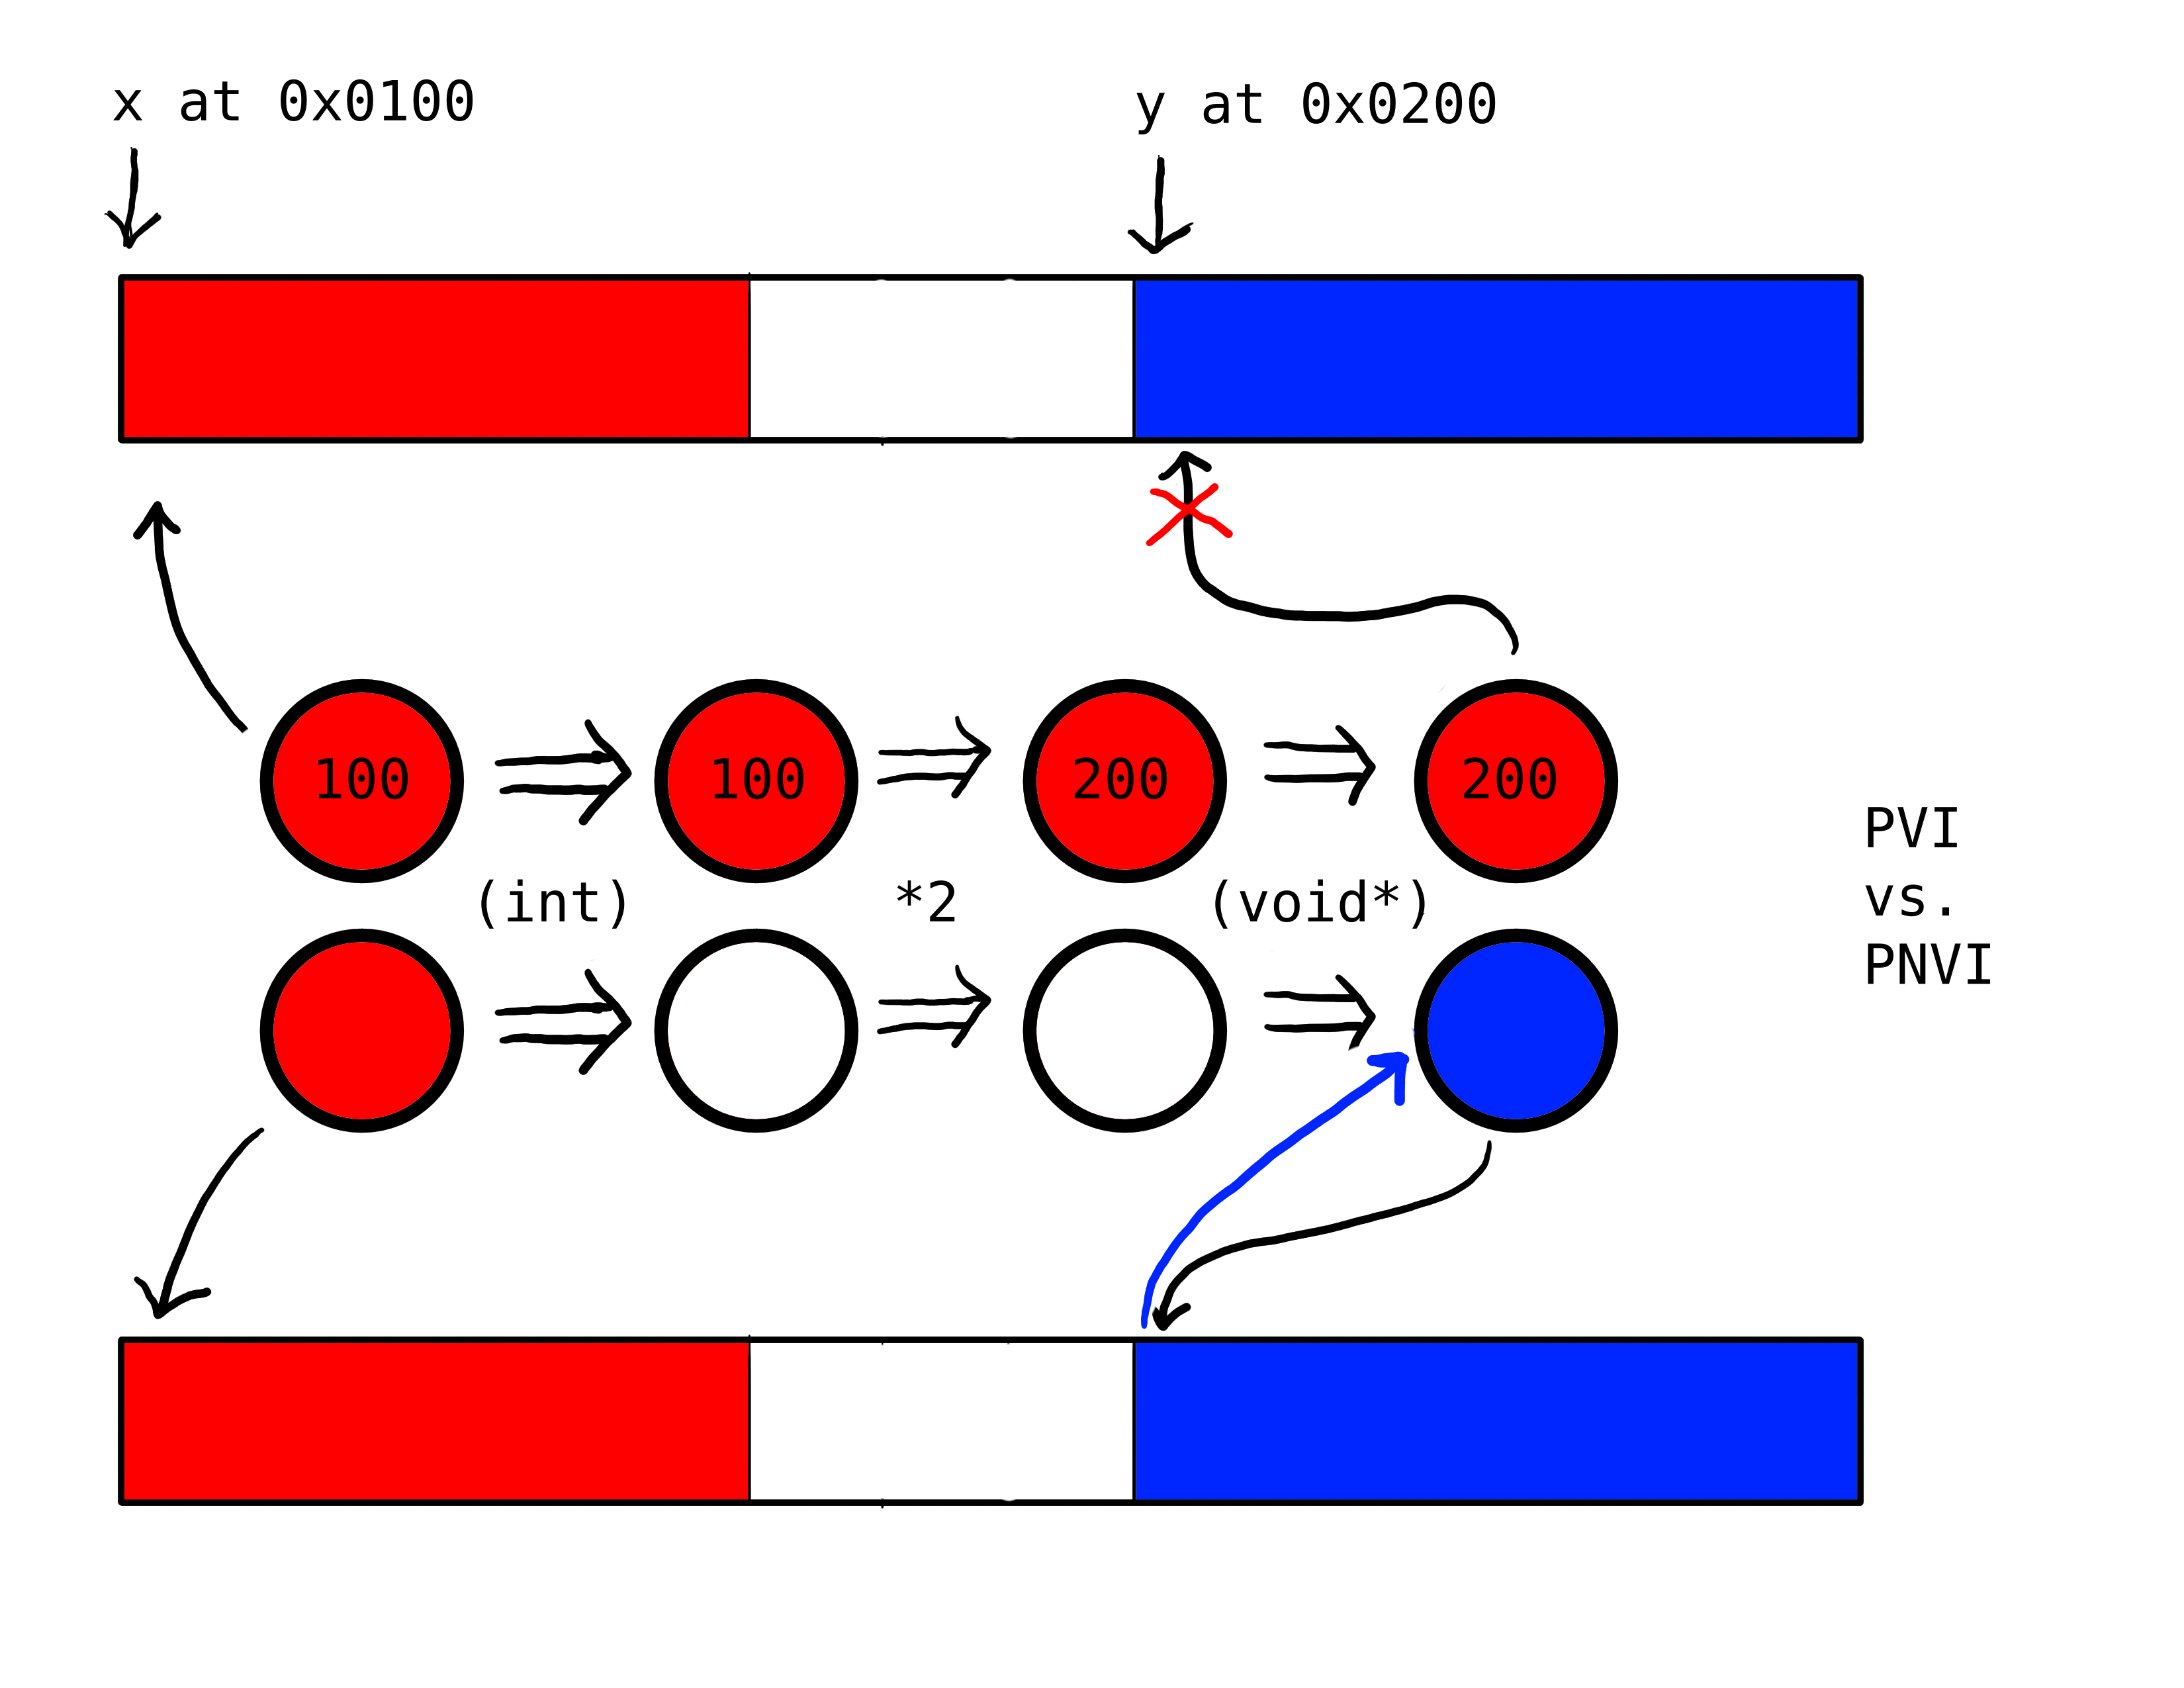
\includegraphics[width=.6\textwidth]{PVIvsPNVI.png}
%  \caption{Integer-pointer casts in PVI and PNVI}
%  \label{fig:PVI-PNVI}
%\end{figure}

%We will aim to prove that for any program, if it is run in both the PVI semantics
%and in Tagged C with our PVI policy, it either produces identical output, or it is both
%undefined in the PVI semantics and failstops in Tagged C. Likewise for PNVI, except that
%some UB in PNVI is non-deterministic, and we only require that it failstop in an execution
%that would {\it reach} the UB.

%In PNVI, the basic provenance model remains the same as PVI, so we can reuse most of the
%same rules. The primary difference is what happens when we cast a pointer to an integer.
%In PVI, tags are propagated as normal.
%To support PNVI, we need the {\it cast} expression to update the tags of a pointer
%being cast to an integer and vice versa. We add two special-case steps to reflect this.

%\judgmenttwo{\optional{\(\mem[p]_{|ty|} = \_@\vt_2 @ \lt\)}}
%            {\(\trule{\picasttres}{\picastt}\)}
%            {\(\defestate{\cast{int}{\val{p}{\pt}}}{\tptr{ty}} \longrightarrow
%              \defestate{\val{p}{vt}}{int}\)}

%\judgmenttwo{\optional{\(\mem[p]_{|ty|} = \_@\vt_2 @ \lt\)}}
%            {\(\trule{\ipcasttres}{\ipcastt}\)}
%            {\(\defestate{\cast{int}{\val{p}{\pt}}}{\tptr{ty}} \longrightarrow
%              \defestate{\val{p}{vt}}{int}\)}

%For casting an integer to a pointer, we don't need the optional ``peek'' at the memory that it points to.
%We simply clear the tag on the resulting integer. On the other hand, when casting back to a pointer,
%we need to check the color of the object that it points to.

%\begin{minipage}{0.34\textwidth}
%\[\begin{aligned}
%\truledef{\picastt}
%\settag{\PCT'}{\PCT}
%\settag{\vt}{N}
%\end{aligned}\]
%\end{minipage}
%\begin{minipage}{0.65\textwidth}
%\[\begin{aligned}
%\truledef{\ipcastt}
%\assert{\exists t . \forall \lt \in \lt . \lt = t \land t \not = N}
%\settag{\PCT'}{\PCT}
%\settag{\pt}{t}
%\end{aligned}\]
%\end{minipage}

%\paragraph{Realizing the Integer-Pointer Cast}

\subsection{Secure Information Flow}
\label{sec:SIF}

Our final example policy will be a more realistic version of our first:
{\em secure information flow (SIF)}. SIF is described in Denning and Denning
\cite{Denning77:SecureInformationFlow}, and is part of a larger family of policies
known as {\em information flow control} (IFC.) This family of policies deal entirely with enforcing
higher-level security concerns, regardless of whether the code that they protect contains
errors or undefined behaviors. We will give an example of a single policy in the family.
Our introductory example was an instance of {\em confidentiality}, so now we will discuss
{\em integrity}: preventing insecure input from influencing secure behavior.
In this code, a malformed user input is accidentally appended to an sql query without sanitization:

\begin{verbatim}
void sanitize(char* in, char* out);
char* sql_query(char* query);

void get_data() {
  char[20] name;
  char[20] name_san;
  char[100] query = "select address where name =";

  scanf("%19f", name);
  sanitize(name, name_san);
  strncat(query, name, strlen(name));
  
  sprintf(buf, sql_query(query));
  return;
}
\end{verbatim}

This function sanitizes its input {\tt name}, then appends the result to an appropriate SQL
query, storing the result in {\tt buf}. But, in the default case, the programmer has accidentally
used the unsanitized string! This creates the opportunity for an SQL injection attack: a caller
to this function could (presumably at the behest of an outside user) call it with {\tt field} of
3 and {\tt name} of ``Bobby; drop table;''.

The fact that the input can be sanitized also makes this an {\em intransitive} policy:
information may flow from {\tt scanf} to {\tt sanitize}, and from {\tt sanitize} to
{\tt sql\_query}, but not directly from {\tt scanf} to {\tt sql\_query}.

\begin{figure}

  \begin{minipage}{0.3\textwidth}
    \color{blue}
    \begin{align*}
      \tau ::= & \high \\
      & \low \\
      & \pctaint{f}{d}{Ls} & d \in \mathbb{N}, ~ Ls \in \mathit{list} ~ id \\
    \end{align*}
  \end{minipage}
  \begin{minipage}{0.69\textwidth}
    \[|\gentag| \triangleq
    \begin{cases}
      \high & \textnormal{if } \gentag = \high \textnormal{ or } \gentag = \pctaint{f}{0}{\varepsilon} \\
      \low & \textnormal{otherwise} \\
    \end{cases}\]
    %
    \[\gentag_1 \sqcap \gentag_2 \triangleq
    \begin{cases}
      \high & \textnormal{if } |\gentag_1| = |\gentag_2| = \high \\
      \low & \textnormal{otherwise} \\
    \end{cases}\]
  \end{minipage}

  \begin{minipage}{0.54\textwidth}
    \storetruleblock
        {let \(\pctaint{f}{d}{Ls} := \PCT\) in \\
          \(\PCT' := \PCT\) \\
          \(\lt' := \lt\) \\
          \caseofthree{\(f\)}
                      {\(\mathtt{scanf}\)}{\(\vt':=\low\)}
                      {\(\mathtt{sanitize}\)}{\(\vt':=\high\)}
                      {\(\underline{\hspace{3em}}\)}
                      {\(\vt' := \PCT \sqcap \vt \sqcap \pt\)}}
  \end{minipage}
  \begin{minipage}{0.45\textwidth}
    \loadtruleblock
        {let \(\pctaint{f}{d}{Ls} := \PCT\) in \\
          \caseoftwo{\(f\)}
                    {\(\mathtt{sql\_query}\)}{\(\mathbf{assert} ~ \vt \sqcap \pt = \high\) \\ & & \(\vt' := \vt\)}
                    {\(\underline{\hspace{3em}}\)}{\(\vt' := \vt\)}}

    \binoptruleblock{\(\vt' := \vt_1 \sqcap \vt_2\)}
  \end{minipage}

\caption{SIF Policy: Tags and Selected Rules}
\label{fig:sif1}
\end{figure}

Since we care about a single source\apt{??}, we can once again use a pair of \(\high\)
and \(\low\) tags, although in this case we aim to prevent \(\low\)-integrity
data from flowing to \(\high\)-integrity locations.
We additionally need to carry significant information on the PC tag,
so we define a third type of tag, written using the constructor {\sc \color{blue} pc},
which carries (1) the current function identifier, (2) a natural number to record
a count of tainted expression scopes, and (3) a stack of label identifiers to record
the join points of tainted statement scopes. We will discuss (2) and (3) in detail below.
Initially, the PC tag is \(\pctaint{f}{0}{\varepsilon}\).

Selected tag rules for expressions are given in \cref{fig:sif1}. We define two operators on tags:
the ``join'' operator \(\sqcap\) takes the higher of two security levels, and the ``reduce''
operator \(| \cdot |\) converts a PC tag into a security level, \(\high\) or \(\low\).
The function {\tt scanf} taints all of its writes by marking them \(\low\). \apt{I thought we'd agreed
  that this was an overly heavy-handed way to make {\tt scanf} taint the input. However...} This extends to
its return value in \(\rettname\) as well (not shown).\apt{But it doesn't have a return value! And how would we express
  that it should taint its (second) argument?}
Similarly, all outputs of {\tt sanitize} are tagged \(\low\), so that when it copies \(\high\)-tagged data into its
output buffer, we consider those data safe.\apt{But again, how is this expressed in a policy? For examples, baybe better to avoid
passing data back via args (although of course we should have a story for that).}

In this scenario, our policy aims to prevent {\tt sql\_query} from recieving tainted data.
For this reason, we failstop if {\tt sql\_query} would load a \(\low\) value.\apt{Ditto on this being
  a heavy-handed and indirect scheme. Just want to say that the {\tt query} is $\low$.}

\paragraph*{Implicit Flows}

This is where the other components of the PC tag come into play. We perform a program
transformation introducing the labels of all join points explicitly, so that in
\cref{fig:ifthenelse}, {\tt J} is an explicit label in the code, if it wasn't already.\apt{
  Clarify that this ``transformation'' is strictly internal/conceptual; maybe put forward pointer to para at end of this section
  (or more that here)?}
We introduce an internal form of each conditional statement
(if, switch, while, do-while, and for) that takes as an extra parameter the label of
that conditional's join point. As seen in \cref{fig:SIFconditionals}, the
\(\splittname\) tag rule takes this label as an optional parameter and, if
the conditional branches on a low value, pushes the join point to the stack.
Then the \(\labeltname\) rule checks if execution has reached a join point and
if it has, removes it from the stack. A PC tag can only reduce to \(\high\)
if its stack is empty.

Branching expressions work similarly, except that the join point occurs at a different
internal expression form: the parenthetical expression. For example, the expression
{\tt 1 ? a : b} reduces to the parenthetical {\tt (a)}.\apt{This requires a much deeper understanding
  of reduction semantics than anything else in the paper -- can that be avoided?} The \(\exprjointname\) rule
applies when {\tt a} is fully reduced and the semantics throw away the parentheses.
Because expressions are nested, we only need to keep track of how deep execution has
gone since the first time it branched on a \(\low\) value, by incrementing and decrementing
the depth \(d\). \apt{This is obscure.} \(\exprjointname\) also tags the result of the expression.\apt{This
  seems too trivial to note in the text. Except: what \emph{is} the reason for joining with P in the paritcular rule shown?}

We assume a {\em termination-insensitive} setting \cite{Askarov08:TINILeaks}, in which
we allow an observer to glean information by the termination or non-termination of
the program. This is a necessary limitation of an enforcement mechanism that halts
execution. Having accepted this limitation, we may apply the same analysis to loops
as well as conditionals.

\begin{figure}
  \begin{minipage}{0.55\textwidth}
    \splittruleblock{
      \caseoftwo{\(\PCT, \vt\)}
                {\(\pctaint{f}{d}{Ls}, \low\)}{\(\PCT' := \pctaint{f}{d}{(L::Ls)}\)}
                {\(\underline{~~~}, \high\)}{\(\PCT' := \PCT\)}
    }
    \labeltruleblock{
      \caseoftwo{\(\PCT\)}
                {\(\pctaint{f}{d}{Ls}\)}{
                  let \({\color{blue} Ls'} = \mathit{pop\_all} ~ {\color{blue} \LN ~ Ls}\) in \\
                  & &      \(\PCT' := \pctaint{f}{d}{Ls'}\)
                }
                {\(\underline{~~~}\)}{\(\PCT' := \PCT\)}
    }
  \end{minipage}
  \begin{minipage}{0.35\textwidth}
    \exprsplittruleblock{
      \caseoftwo{\(\PCT, \vt\)}
                {\(\pctaint{f}{d}{Ls}, \low\)}{\(\PCT' := \pctaint{f}{(d+1)}{Ls}\)}
                {\(\underline{~~~}, \high\)}{\(\PCT' := \PCT\)}
    }

    \exprjointruleblock{
      \(\vt' := \vt \sqcap \PCT\) \\
      \caseoftwo{\(\PCT\)}
                {\(\pctaint{f}{(d+1)}{Ls}\)}{\(\PCT' := \pctaint{f}{d}{Ls}\)}
                {\(\underline{~~~}\)}{\(\PCT' := \PCT\)}
    }
  \end{minipage}
  
  \caption{SIF Conditionals}
  \label{fig:SIFconditionals}
\end{figure}

Of course, code does not generally come with labeled join points, and they must be associated
with their split points. We introduce additional forms of the if, while, do-while, for, and switch
statements which carry an additional label, and perform some preprocessing to associate these
with new labels in the source code. This preprocessing step generates the program's
control flow graph and, for each branch, identifies its immediate post-dominator. That
node is labeled with  a fresh identifier, and the same identifier is added to the original
conditional statement.

%\begin{figure}
%  \begin{subfigure}{0.49\textwidth}
%\begin{verbatim}
%int f(bool secret) {
%    int public1=1;
%    int public2;
%
%S:  while (secret) {
%b1:     public1 = 1;
%        secret = false;
%    }
%
%J:  public2 = 42;
%
%    return public2;
%}
%\end{verbatim}
%  \caption{Leaking via while statements}
%  \label{fig:while}
%  \end{subfigure}
%  \begin{subfigure}{0.5\textwidth}
%    \begin{tikzpicture}
%      [ initial text={}, initial distance=4em,
%        accepting/.style=accepting by arrow,
%        accepting distance=4em
%      ]
%      \node[state,initial]    (S)                        {$S$};
%      \node[state]            (b_1) [above right=of S]   {$b_1$};
%      \node[state,accepting]  (J)   [below right=of b_1] {$J$};

%      \path[->] (S)   edge               node  {}  (b_1)
%                      edge               node  {}  (J)
%                (b_1) edge [bend right] node  {}  (S);
%    \end{tikzpicture}
%  \end{subfigure}
%  
%\end{figure}

%\begin{figure}
%  \begin{subfigure}{0.25\textwidth}
%\begin{verbatim}
%int f(bool secret) {
%    int public1, public2;

%    while (secret) {
%        goto b1;
%    }

%b2: public1 = 1;
%    goto J;

%b1: public1 = 1;

%J:  public2 = 42;
%    return public2;
%}
%\end{verbatim}
%  \end{subfigure}
%  \begin{subfigure}{0.74\textwidth}
%    \begin{tikzpicture}
%      [ initial text={}, initial distance=3em,
%        accepting/.style=accepting by arrow,
%        accepting distance=3em
%      ]
%      \node[state,initial]    (S)                              {$S$};
%      \node[state]            (inside) [above right=of S]      {};
%      \node[state]            (b_2)    [below right=of inside] {$b_2$};
%      \node[state]            (b_1)    [right=of b_2]          {$b_1$};
%      \node[state,accepting]  (J)      [right=of b_1]          {$J$};

%      \path[->] (S)   edge              node  {}  (inside)
%                      edge              node  {}  (b_2)
%                (inside) edge [bend left] node {} (b_1)
%                (b_1) edge              node  {}  (J)
%                (b_2) edge [bend right] node  {}  (J);
%    \end{tikzpicture}
%  \end{subfigure}
  
%  \caption{Cheating with go-tos}
%  \label{fig:forbreak}
%\end{figure}
%\begin{figure}
%  \begin{subfigure}{0.3\textwidth}
%    \begin{tikzpicture}
%      [ initial text={}, initial distance=1em,
%        accepting/.style=accepting by arrow,
%        accepting distance=1em
%      ]
%      \node[state,initial]    (do)                             {do};
%      \node[state,accepting]  (S) [right=of do]                {\(S\):test};

%      \path[->] (do)   edge              node  {}  (S)
%                (S)    edge [bend left]  node  {}  (do);
%    \end{tikzpicture}
%    \subcaption{Do-while}
%  \end{subfigure}
%  \begin{subfigure}{0.3\textwidth}
%    \begin{tikzpicture}
%      [ initial text={}, initial distance=1em,
%        accepting/.style=accepting by arrow,
%        accepting distance=1em
%      ]
%      \node[state,initial]    (init)                             {init};
%      \node[state,accepting]  (S)    [right=of init]             {\(S\):test};
%      \node[state]            (do)   [above=of S]                {do};
%      \node[state]            (post) [left=of do]                {post};
      
%      \path[->] (init)   edge              node  {}  (S)
%                (S)      edge              node  {}  (do)
%                (do)     edge              node  {}  (post)
%                (post)   edge              node  {}  (S);
%    \end{tikzpicture}
%    \subcaption{For}
%  \end{subfigure}
%  \begin{subfigure}{0.3\textwidth}
%    \center
%    \begin{tikzpicture}
%      [ initial text={}, initial distance=1em, initial above,
%        accepting/.style=accepting by arrow,
%        accepting distance=1em, node distance=2em, inner sep=1pt
%      ]
%      \node[state,initial]    (switch)                           {\(S\):switch};
%      \node[state]            (case1)    [below left=of switch]  {};
%      \node[state]            (case2)    [right=of case1]        {};
%      \node[state]            (default)  [right=of case2]        {def};
%      \node                   (after)    [right=of default]      {};

%      \path[->] (switch)  edge              node  {}  (case1)
%                          edge              node  {}  (case2)
%                          edge              node  {}  (default)
%                (default) edge              node  {}  (after)
%                (case1)   edge [bend right] node  {}  (after)
%                (case2)   edge [bend right] node  {}  (after);

%      \path[dotted,->] (case1) edge              node  {}  (case2)
%                (case2) edge              node  {}  (default);
                         
%    \end{tikzpicture}
%    \subcaption{Switch}
%  \end{subfigure}
  
%  \caption{Remaining Branch Statements}
%  \label{fig:rest}
%\end{figure}


\section{Implementing Tagged C with PIPE}
\label{sec:optionals}

Chhak et al. \cite{Chhak21:Tagine} introduce a verified compiler from a toy
high-level language with tags
to a control-flow-graph-based intermediate representation of a PIPE-based
ISA. It is a proof-of-concept of compilation from a source language's tag policy to
realistic hardware. Everything in a PIPE system carries tags, including instructions. 
Instruction tags are statically determined at compile-time, so they can carry data about source-level
control points in the corresponding assembly. This means that PIPE can emulate any given Tagged C
policy by running two policies in parallel: a basic stack-and-function-pointer-safety policy to mimic Tagged C's
high-level control-flow, and the source-level policy as written.

Chhak et al.'s general strategy for mapping Tagged C's tag rules sometimes requires adding extra
instructions to the generated code. A Tagged-C control point
may require a tag from a location that is not read under a normal compilation scheme, or must update tags
in locations that would otherwise not be written. Such instructions are unnecessary overhead if the policy
doesn't meaningfully use the relevant tags.

To mitigate this, control points whose compilation would add potentially extraneous instructions
take optional parameters or return optional results. We will explain how the rule should be
implemented in the target if the options are used.
Optional inputs and outputs are marked with boxes. If a policy does not make use of the options, it will
be sound to compile without the extra instructions.

\section{Evaluation}
\label{sec:evaluation}

Tagged C aims to combine the flexibility of tag-based architectures with the abstraction
of a high-level language. How well have we achieved this aim?

[Here we list criteria and evaluate how we fulfilled them]

\begin{itemize}
\item Flexibility: we demonstrate three policies that can be used alone or in conjunction
\item Applicability: we support the full complement of C language features and give definition
  to many undefined C programs
\item Practical security: our example security policies are based on important security concepts
  from the literature
\end{itemize}

\subsection{Limitations of the Tag Mechanism}

By committing to a tag-based mechanism, we do restrict the space of policies that Tagged C
can enforce. In general, a reference monitor can enforce any policy that constitutes a
{\em safety property}---any policy whose violation can be demonstrated by a single finite
trace. This class includes such policies as ``no integer overflow'' and ``pointers are always in-bounds,''
which depend on the values of variables. Tag-based monitors cannot enforce any policy that
depends on the value of a variable rather than its tags.

\section{Related Work}

\paragraph{Reference Monitors}

The concept of a reference monitor was first introduced fifty years ago~\cite{Anderson72:PlanningStudy}
as a tamper-proof and verifiable subsystem that checks every security-relevant operation in a system to
ensure that it conforms to a security {\em policy} (a general specification of acceptable behavior~\cite{Goguen82:SecurityPolicies}).

A reference monitor can be implemented at any level of a system. An {\em inline reference monitor}\cite{??}
is a purely compiler-based system that inserts checks at appropriate places in the code.
Alternatively, a reference monitor might be embedded in the operating system, or in an interpreted
language's runtime. A {\em hardware reference monitor} instead provides primitives at the ISA-level
that accelerate security and make it harder to subvert.

Programmable Interlocks for Policy Enforcement (PIPE) \cite{Dhawan14:PUMP} is a hardware extension
that uses {\em metadata tagging}. Each register and each word of memory is associated with
an additional array of bits called a tag. The policy is decomposed into a set of {\em tag rules}
that act in parallel with each executing instruction, using the tags on its operands to
decide whether the instruction is legal and, if so, determine which tags to place on its results.
PIPE tags are large relative to other tag-based hardware, giving it the flexibility
to implement complex policies with structured tags, and even run multiple policies at once.

Other hardware monitors include Arm MTE, STAR, and CHERI.
Arm MTE aims to enforce a narrow form of memory safety using 4-bit tags, which distinguish adjacent objects
in memory from one another, preventing buffer overflows, but not necessarily other memory violations.
[TODO: read the Binghamton paper, figure out where they sit here.] 

CHERI is capability machine [TODO: cite OG CHERI]. In CHERI, capabilities
are ``fat pointers'' carrying extra bounds and permission information, and capability-protected
memory can only be accessed via a capability with the appropriate privilege. This is a natural
way to enforce spatial memory safety, and techniques have been demonstrated for enforcing
temporal safety \cite{NWF20:Cornucopia}, stack safety \cite{Skorstengaard19:stktokens},
and compartmentalization [TODO: figure out what to cite], with varying degrees of ease and
efficiency. But CHERI cannot easily enforce notions of security based on dataflow,
such as Secure Information Flow.

In this paper, we describe a programming language with an abstract reference monitor.
We realize it as an interpreter with the reference monitor built in, and envision
eventually compiling to PIPE-equipped hardware. An inlining compiler would also be plausible.
As a result of this choice, our abstract reference monitor uses a PIPE-esque notion of
tags.\apt{A grot-esque coinage.}

\paragraph{Aspect Oriented Programming}

[TODO: do forward search from original AOP paper]

\section{Future Work}
\label{sec:futurework}

We have presented the language and a reference interpreter, built on top of the CompCert interpreter
\cite{Leroy09:CompCert}, and three example policies. There are several significant next-steps.

\paragraph{Compilation}

An interpreter is all well and good\apt{too informal}, but a compiler would be preferable for many reasons.
A compiled Tagged C could use the hardware acceleration of a PIPE target, and could more easily
support linked libraries, including linking against code written in other languages.
The ultimate goal would be a fully verified compiler, but that is a very long way off\apt{too informal}.


\paragraph{Language Proofs}

There are a couple of properties of the language semantics itself that we would like to prove.
Namely (1) that its behavior (prior to adding a policy) matches that of CompCert C and
(2) that the behavior of a given program is invariant under all policies up to truncation due
to failstop.

\paragraph{Policy Correctness Proofs}

For each example policy discussed in this paper, we sketched a formal specification for the
security property it ought to enforce. A natural continuation would be to prove the correctness
of each policy against these specifications.

\paragraph{Policy DSL}

Currently, policies are written in Gallina, the language embedded in Coq. This is fine for a
proof-of-concept, but not satisfactory for real use. We plan to develop a domain-specific policy
language to make it easier to write Tagged C policies.

\bibliographystyle{splncs04}
\bibliography{taggedc.bib}

\appendix

\section{Syntax}

Tagged C has the full complement of typical C expressions (\cref{fig:expr}). \(\val{v}{\vt}\),
\(\loc{p}{\pt}\), and \(\paren{\expr}{\type}\) are internal forms.
A constant \(c\) in the concrete syntax is transformed into \(\val{c}{\constt}\),
and in general \(\val{v}{\vt}\) is a fully-reduced right-hand value. \(\loc{p}{\pt}\)
is a fully-reduced left-hand value that represents the address of a variable.
\(\paren{\expr}{\type}\) is the result of a conditional or shortcutting
expression, with \(\ty\) being a type annotation in case the result needs to
be cast.

\begin{figure}
  \[\begin{aligned}
  \expr ::= & \val{v}{\vt} & \textnormal{Value} \\
  | & \var{x} & \textnormal{Variable} \\
  | & \field{\expr}{id} & \textnormal{Field} \\
  | & \valof{\expr} & \textnormal{Load from Object} \\
  | & \deref{\expr} & \textnormal{Dereference Pointer} \\
  | & \addrof{\expr} & \textnormal{Address of Object} \\
  | & \unop{\odot}{\expr} & \textnormal{Unary Operator} \\
  | & \binop{\oplus}{\expr_1}{\expr_2} & \textnormal{Binary Operator} \\
  | & \cast{\expr}{ty} & \textnormal{Cast} \\
  | & \condition{\expr_1}{\expr_2}{\expr_3} & \textnormal{Conditional} \\
  | & \sizeof{ty} & \textnormal{Size of Type} \\
  | & \alignof{ty} & \textnormal{Alignment of Type} \\
  | & \assign{\expr_1}{\expr_2} & \textnormal{Assignment} \\
  | & \assignop{\oplus}{\expr_1}{\expr_2} & \textnormal{Operator Assignment} \\
  | & \postinc{\oplus}{\expr} & \textnormal{Post-Increment/Decrement} \\
  | & \comma{\expr_1}{\expr_2} & \textnormal{Expression Sequence} \\
  | & \call{\expr_f}{\overline{\expr}_{args}} & \textnormal{Function Call} \\
  | & \loc{l}{\lt} & \textnormal{Memory Location} \\
  | & \paren{\expr}{ty}{\gentag} & \textnormal{Parenthetical with Optional Cast} \\
  \end{aligned}\]
  \caption{Expression Syntax}
  \label{fig:expr}
\end{figure}

Some common C expressions are derived forms. An array index expression,
\(\expr_1[\expr_2]\) expands to \(\deref{\binop{+}{\expr_1}{\expr_2}}.
The pre-increment  expression \(++\expr\) expands to
\(\assign{\expr}{\binop{+}{\expr}{1@\constt}}\), and likewise for pre-decrement.

Similarly, statements cover the full C standard. Conditional statements
carry optional labels as internal forms, so that an if statement in the
concrete syntax becomes \(\sifthenelse{\expr}{\stmt_1}{\stmt_2}{\bot}\).

\begin{figure}
  \begin{subfigure}[t]{0.3\textwidth}
    \[\begin{aligned}
    \stmt ::= & \sskip \\
    | & \sdo{\expr} \\
    | & \sseq{\stmt_1}{\stmt_2} \\
    | & \sifthenelse{\expr}{\stmt_1}{\stmt_2}{L} \\
    | & \swhile{\expr}{\stmt}{L} \\
    | & \sdowhile{\expr}{\stmt}{L} \\
    | & \sfor{\stmt_1}{\expr}{\stmt_2}{\stmt_3} \\
    | & \sbreak \\
    | & \scontinue \\
    | & \sreturn \\
    | & \sswitch{\expr}{\overline{(L,\stmt)}} \\
    | & \slabel{L}{\stmt} \\
    | & \sgoto{L} \\    
    \end{aligned}\]
  \end{subfigure}
  \begin{subfigure}[t]{0.69\textwidth}
  \end{subfigure}
  \caption{Tagged C Abstract Syntax}
  \label{fig:syntax}
\end{figure}

\section{States}

States can be of several kinds, denoted by their script prefix: a {\em general state} \(\mathcal{S}(\dots)\),
an {\em expression state} \(\mathcal{E}(\dots)\), a {\em call state} \(\mathcal{C}(\dots)\), or a
{\em return state} \(\mathcal{R}(\dots)\). Finally, the special state {\em failstop} (\(\mathcal{F}(\dots)\))
represents a tag failure, and carries the state that produced the failure.
[Allison: to whatever degree you've figured out what is useful here by publication-time, we can
  tune this to be more specific.]

In the below definition, memories are ranged over by \(\mem\), local environments by
\(\lenv\), and continuations by \(\cont\).

\[\begin{aligned}
S ::= & \sstate{\PCT}{\mem}{\stmt}{\cont} \\
| & \estate{\PCT}{\mem}{\expr}{\cont} \\
| & \cstate{f}{\PCT}{\mem}{\lenv}{f'}{\overline{\val{v}{\vt}}}{\cont} \\
| & \rstate{\PCT}{\mem}{\genv}{\lenv}{\val{v}{\vt}}{\cont} \\
| & \fstate{S} \\
\end{aligned}\]


States in general contain a memory, a local environment, and a continuation.

\subsection{Memories}

\subsection{Environments}

\subsection{Continuations}
\label{app:continuations}

A continuation acts like a stack of pending operations. The base of the stack is
\(\kemp\). \(\mathit{Kdo}\) indicates that a do statement is evaluating an expression.
\(\mathit{Kseq}\) with parameter \(\stmt\) indicates that, after the current statement
is done executing, \(\stmt\) is next. \(\mathit{Kif}\) means that execution is evaluating
the test expression of an if statement, and its parameters are the branches of the
if. Similarly, the test continuations for while, do-while, and for loops indicate that
the test expression is being evaluated. The associated loop continuations indicate that
execution is in the loop body. They continuations carry all of the information of the original
loop.

\[\begin{split}
\cont ::= & \kemp \\
| & \kdo{\cont} \\
| & \kseq{\stmt}{\cont} \\
| & \kif{\stmt_1}{\stmt_2}{L}{\cont} \\
| & \kwhiletest{\expr}{\stmt}{L}{\cont} \\
| & \kwhileloop{\expr}{\stmt}{L}{\cont} \\
| & \kdowhiletest{\expr}{\stmt}{L}{\cont} \\
| & \kdowhileloop{\expr}{\stmt}{L}{\cont} \\
| & \kfor{\expr}{\stmt_2}{\stmt_3}{L}{\cont} \\
| & \kforpost{\expr}{\stmt_2}{\stmt_3}{L}{\cont} \\
\end{split}\]


\section{Initial State}

Given a list \(xs\) of variable identifiers \(id\) and types
\(ty\), a program's initial memory is defined by iteratively allocating each one
in memory and updating the global environment with its base address, bound, type,
and a static identity tag. Let \(|ty|\) be a function from types to their sizes
in bytes. The memory is initialized \(\vundef@\vt@\lt\)
for some \(\vt\) and \(\lt\), unless given an initializer.
Let \(\mem_0\) and \(\genv_0\) be the initial (empty) memory and environment.
The parameter \(b\) marks the start of the global region.

%Since we don't need to initialize tags in memory dynamically, our rule for
%selecting these tags can cover the entire initialization of the memory with arbitrary
%granularity. We represent this as a list of tags of length \(|ty|\).

\[\mathit{globals} ~ xs ~ b =
\begin{cases}
  (\mem_0, \genv_0) & \textnormal{if } xs = \varepsilon \\
  (\mem[p \dots p+|ty| \mapsto \vundef@\vt@\lt]_{|ty|}, & \textnormal{if } xs = (id,ty)::xs' \\
  ~ \genv[id \mapsto (\mathit{p, p+|ty|,ty,\pt})]) & \textnormal{and } \trule{\globaltres}{\globalt} \\
  & \textnormal{where } (\mem,\genv) = \mathit{globals} ~ xs' ~ (b + |ty|) \\
\end{cases}\]

\section{Step Rules}
\label{app:rules}

\subsection{Sequencing rules}

\sequencing

\subsection{Conditional rules}

\conditionals

\subsection{Loop rules}

\loops

\subsection{Contexts}
\label{app:contexts}

Our expression semantics are contextual. A context \(\ctx[\expr]_k\) is a function from an
expression to an expression, with a ``kind'' flag \(k\) (left-hand or right-hand, \(\lh\) or \(\rh\)).

\[\begin{aligned}
\ctx{\expr}_\lh ::= \\
| & \expr & \\ % ctx_top
| & \deref{\ctx{\expr}_\rh} \\ % ctx_deref
| & \field{\ctx{\expr}_\rh}{id} \\ % ctx_field
\end{aligned}\]

\[\begin{aligned}
\ctx{\expr}_\rh ::= \\
| & \expr & \\ % ctx_top
| & \valof{\ctx{\expr}_\lh} \\ % ctx_rvalof
| & \addrof{\ctx{\expr}_\lh} \\ % ctx_addrof
| & \unop{\odot}{\ctx{\expr}_\rh} \\ % ctx_unop
| & \binop{\oplus}{\ctx{\expr_1}_\rh}{\expr_2} \\ % ctx_binop_left
| & \binop{\oplus}{\expr_1}{\ctx{\expr_2}_\rh} \\ % ctx_binop_right
| & \cast{\ctx{\expr}_\rh}{\type} \\ % ctx_cast
| & \seqand{\ctx{\expr_1}_\rh}{\expr_2} \\ % ctx_seqand
| & \seqor{\ctx{\expr_1}_\rh}{\expr_2} \\ % ctx_seqor
| & \condition{\ctx{\expr_1}_\rh}{\expr_2}{\expr_3} \\ % ctx_condition
| & \assign{\ctx{\expr_1}_\lh}{\expr_2} \\ % ctx_assign_left
| & \assign{\expr_1}{\ctx{\expr_2}_\rh} \\ % ctx_assign_right
| & \assignop{\oplus}{\ctx{\expr_1}_\lh}{\expr_2} \\ % ctx_assignop_left
| & \assignop{\oplus}{\expr_1}{\ctx{\expr_2}_\rh} \\ % ctx_assignop_right
| & \postinc{\oplus}{\ctx{\expr}_\lh} \\ % ctx_postinc
| & \call{\ctx{\expr_1}_\rh}{\overline{\expr_2}} \\ % ctx_call_left
| & \call{\expr_1}{\ctx{\overline{\expr_2}}_\rh} \\ % ctx_call_right
% skipped builtins
| & \comma{\ctx{\expr_1}_\rh}{\expr_2} \\ % ctx_comma
| & \paren{\ctx{\expr}_\rh}{\type}{} \\ % ctx_paren
\end{aligned}\]

A left-hand reduction \(\expr \Rightarrow_\lh \expr'\)
relates an expression to an expression. A right-hand reduction
\((\PCT,\mem,\expr) \Rightarrow_\rh (\PCT',\mem',\expr')\)
relates a triple of PC Tag, memory, and expression to another such triple.
Given these reduction relations, we construct step rules for contexts in
expressions.

%triple of a memory, an expression, and a tag
%might reduces to another such triple as a left-hand, right-hand, or call reduction, written
%\((\mem, \expr, \PCT) \Rightarrow_k (\mem', \expr', \PCT')\),
%based on rules given below. These reductions are embedded in states as follows.

\judgmenttwo{\(\ctx{\expr}_\lh\)}
            {\(\expr \Rightarrow_\lh \expr'\)}
            {\(\defestate{\ctx{\expr}} \longrightarrow \defestate{\ctx{\expr'}}\)}

\judgmenttwo{\(\ctx{\expr}_\rh\)}
            {\((\PCT, \mem, \expr) \Rightarrow_\rh (\PCT', \mem', \expr')\)}
            {\(\defestate{\ctx{\expr}} \longrightarrow \estate{\PCT'}{\mem'}{\ctx{\expr'}}{\cont}\)}
            
All that remains is to give the expression reductions themselves.

\expressions

\subsection{Call and Return Rules}

In order to make a call, we need to reduce the function expression to an \(\floc{\_}\) value, an
abstract location corresponding to a particular function. Then we can make the call.

\callexprstep

When we make an internal call, we need to allocated space for locals and arguments using the helper function
\(\mathit{frame}\).

\[\mathit{frame} ~ xs ~ as ~ \mem =
\begin{cases}
  (\mem''[p \mapsto \vundef@\vt@\lt]_{|ty|}, & \textnormal{if } xs = (id,ty)::xs' \\
  \lenv'[id \mapsto (\mathit{p, p+|ty|,ty,\pt})]) &
  \textnormal{where } (\mem',p) \leftarrow \mathit{stack\_alloc} ~ |ty| ~ \mem, \\
  & \trule{\localtres}{\localt}, \\
  & \textnormal{and } (\mem'',\lenv') = \mathit{frame} ~ xs' ~ as ~ m' \\ 
  \\
  (\mem''[p \mapsto v@\vt'@\lt]_{|ty|}, & \textnormal{if } as = (id,ty,v @ \vt)::as' \textnormal{ and } xs = \varepsilon \\
  \lenv'[id \mapsto (\mathit{p, p+|ty|,ty,\pt})]) &
  \textnormal{where } (\mem',p) \leftarrow \mathit{stack\_alloc} ~ |ty| ~ \mem, \\
  & \trule{\argtres}{\argt}, \\
  & \textnormal{and } (\mem'',\lenv') = \mathit{frame} ~ xs' ~ as ~ m' \\
  \\
  (\mem, \lambda x . \bot) & \textnormal{if } xs = \varepsilon \textnormal{ and } as = \varepsilon \\
\end{cases}\]

\callstep

On the other hand, when we make an external call, we step directly to a return state with some value
being returned and an updated memory. [TODO: talk more about how the tag policy applies in external
  functions, what they can and can't do with tags.]

\extcallstep

Special external functions, such as malloc, just get their own rules.

\mallocstep

And finally, we have the return rules.

\returnstep
\retvalstep
\retnovalstep

%\section{Moved from Intro}

%\sna{I'm organizing our diss tracks into paragraphs that we can cut or move as needed}
%\paragraph*{Why Dynamic?}
  
%  Unfortunately, it is not always possible to fully secure C code before run-time.
%  Ideally, bugs would be quickly identified and then fixed promptly. 
%  That is not always possible for a variety of reasons: bugs may escape detection, 
%  require significant effort to diagnose, or be impractical to fix. 
%  There are many techniques for finding bugs, but there is a shared stumbling block: C is not 
%  well defined. We cannot always agree on when something is a bug in C, especially code using
%  Undefined Behaviors (UB) \cite{defactoC}. Confusion around expected behavior is no small problem. 
%  There are 191 undefined behaviors and 52 unspecified behaviors in the C99 
%  specification \cite{Csmith}. Sometimes these behaviors are benign and skillfully 
%  used by the developer, other times they are unintended and highly dangerous. 
%  Unfortunately the distinction between the two is easily lost. 
%  Discerning expert code review is considered best practice, although it is 
%  rarely perfectly successful \cite{} % https://dl.acm.org/doi/10.1007/978-3-642-36563-8_14 }
%  even if an expert is available at all. Even when there is both consensus 
%  and detection of a bug\apt{??} \amn{we can find it at and we can agree its a problem that should be fixed}, 
%  changing the code may not be possible because  
%  it is in proprietary 3rd party libraries and drivers, or because
%  regulations prohibit changes \cite{Bessey10:Coverity}.

%  \apt{last clause is mysterious} \amn {
%    for example FDA approval used to forbid patching because you'd have to go through recertification. 
%    So healthcare wouldn't patch. SNA pointed out the coverity paper comments on this as a reason for 
%    bugs not getting fixed}

%  \paragraph*{Why C-Level?}
%  Tag-based enforcement in general has a significant body of work at the assembly level, especially
%  PIPE (Programmable Interlocks for Policy Enforcement) \cite{}. However, even at the assembly-level
%  these systems need the compiler to be in the trusted computing base (TCB), as many policies require
%  knowledge of source-level constructs, even ones that do not depend on detailed knowledge of the program's
%  behavior [cite Nick and Andre; anyone else?]. Moving policy-definition to the source level therefore
%  does not expand the TCB and allows C developers to reason about policies in terms of the language that
%  they program in regularly.

%  \paragraph*{Notations}
%  Values are ranged over by \(v\), variable identifiers by \(x\), and function identifiers by \(f\).
%Tags use a number of metavariables: \(t\) ranges over all tags, while we will use
%\(\vt\) to refer to the tags associated with values, \(\pt\) for tags on pointer values
%and memory-location expressions, \(\lt\) for tags associated with memory locations themselves,
%\(\nt\) for ``name tags'' automatically derived from identifiers, \(\PCT\) for the
%global ``program counter tag'' or PC tag.
%An {\it atom} is a pair of a value and a tag, \(\val{v}{\vt}\); the @ symbol should be read
%as a pair in general, and is used when the second object in the pair is a tag.
%Expressions are ranged over by \(\expr\), statements by \(\stmt\), and continuations by \(\cont\).
%The continuations are defined in \cref{app:continuations}, and step rules in \cref{app:rules}.

%A memory is an array of bytes, where each byte is part of an atom.
%Each byte is also associated with a ``location tag'' \(\lt\). When a contiguous region of \(s\) bytes
%starting at location \(l\) comprise an atom \(v@\vt\), and their locations tags comprise the list \(\lts\),
%we write \(\mem[l]_s = v@\vt @\lts\). Likewise, \(\mem[l \dots l + s \mapsto v@\vt @ \lts]_s\)
%denotes storing that many bytes. Visually, we will represent whole atoms in memory as condensed boxes,
%with their location tags separate.

\end{document}
